\chapter{Testing}%%%%%%%%%%%%%%%%%%%%%%%%%%%%%%%%%%%%%%%%%%%%%% 
\label{chap:testing}

In this chapter the various software implementations and design choices made in \refchap{chap:implementation} are used and tested on various aspects. 
This is done to gather the data needed to answer the research questions adequately.
It consists of the sections \refsec{sec:testing:compilation}. \refsec{sec:testing:demo}, \refsec{sec:testing:features}, and \refsec{sec:testing:usability}.


\section{Plugin Compilation \& Utilization}
\label{sec:testing:compilation}

In this section, the tests outlined in \refsec{sec:method:tests:compilation} are performed. 

\subsection{Rust: minimal plugin}

\graphicspath{{../../assets/images/6.1.1/}}

The compilation of the minimum Rust plugin, which exposes a function, a class, and a method, occurred as expected.   
% APPENDIX?
\reffig{fig:minimum-rust-wasm} Shows the source code of this plugin. 
The 'wasm-bindgen' library allows functions and classes to be annotated as 'expose to javascript' with a macro statement. 
This simplifies the compilation process to WebAssembly greatly. 
Due to Rust's macro system, it also creates compile time errors with IDE integration, if a property or class are incompatible to be exposed. 
This aids the construction of a wasm-compatible API. 

This library was compiled to WebAssembly and javascript using 'wasm-pack'. 
This produces multiple artifacts, showcased in \reffig{fig:rust-plugin:compilation-results}. 
This figure also showcases how wasm-pack wraps the functionality: 
The \m{point\_distance} function exposed by the wasm file is wrapped by the javascript file, converting it to look like a regular javascript class.
Keep in mind that as the Interface Type proposal gets accepted as 'standard webassembly' \citep*{wagner_interface_2022}, The javascript or typescript artifacts can be ommited, as this logic will be added to the \m{.wasm} binary itself.
The wasm-pack library is already able to produce a WebAssembly build with interface types included. 
However, as this is not standard WebAssembly yet, it hinders integration with WebAssembly produced from the emscripten compiler, so this study chose against using it.

To check if the result is valid, a small html demo was created to load and use the library (see \reffig{fig:min-rust:demo}).
Note how the JavaScript library wrapping the wasm file looks and works almost like a normal javascript library, the only difference being a 'init' function, which is required to be run before using the library, and the need to free the memory of used object with the \m{free()} method.

To load this project into Geofront, a reference to the path of the compilation artifacts must be specified within the Geofront GUI, shown in \reffig{fig:min-rust-plugin-import}.
A local path was used for convenience, instead of publishing this demo to npm, and accessing it via a \ac{CDN}.

\reffig{fig:rust-plugin-on-canvas:1} shows how all functions in this demo are loaded correctly, and \reffig{fig:rust-plugin-on-canvas:2} shows that the functions indeed work as expected to create two Graphs. 
Note how the parameter names and Types are also loaded, indicated by the names visualized at the input and output of the nodes.
This is thanks to the 'd.ts' file of \reffig{fig:rust-plugin:compilation-results}.

\begin{figure}
\begin{code}
use wasm_bindgen::prelude::*;

#[wasm_bindgen]
pub fn add(left: f32, right: f32) -> f32 {
    left + right
}

#[wasm_bindgen]
pub struct Point {
    pub x: f32,
    pub y: f32,
}

#[wasm_bindgen]
impl Point {

    pub fn new(x: f32, y: f32) -> Point {
        Point { x, y }
    }

    pub fn distance(&self, other: &Point) -> f32 {
        ((self.x - other.x).powi(2) + (self.y - other.y).powi(2)).powf(0.5) 
    }
}
\end{code}
\centering
\caption{Rust: Minimum WebAssembly example}
\label{fig:minimum-rust-wasm}
\end{figure}

\begin{figure}
  \centering
  \begin{subfigure}{0.45\linewidth}
    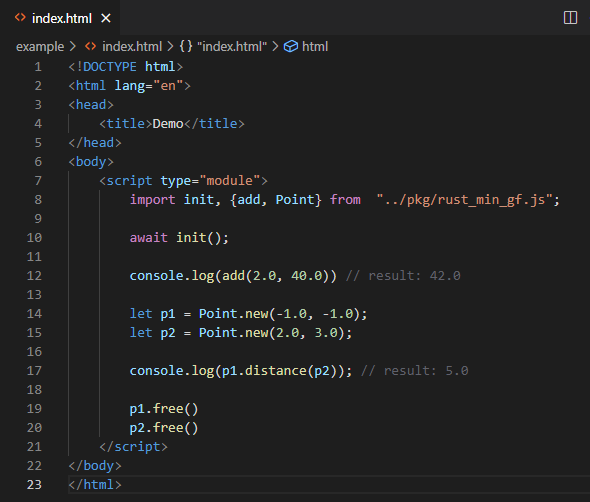
\includegraphics[width=\linewidth]{9.PNG}
    \centering
  \end{subfigure}%
  \qquad
  \begin{subfigure}{0.45\linewidth}
    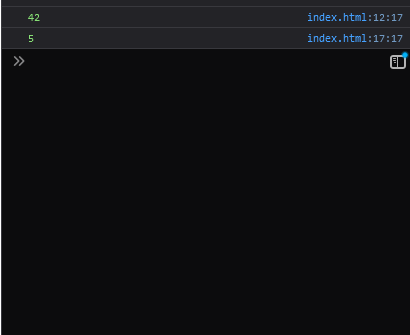
\includegraphics[width=\linewidth]{result.png}
    \centering
  \end{subfigure}%
\caption{Web demo using the WebAssembly build}
\label{fig:min-rust:demo}
\end{figure}

\begin{figure}
  \centering
  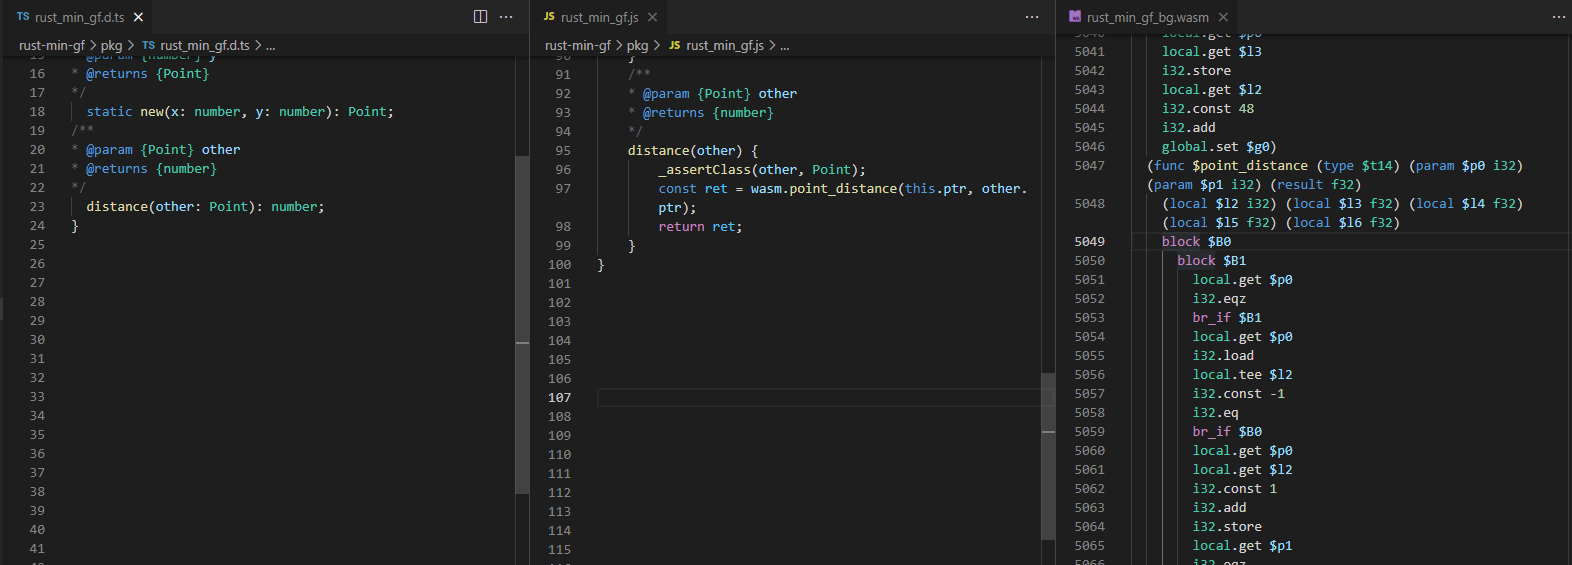
\includegraphics[width=\linewidth]{13.PNG}
  \caption[compilation artifacts]{wasm-pack Compilation artifacts: A Typescript Declaration file, a javascript file, and a WebAssembly binary, visualized as WebAssembly Text (WAT). }
  \label{fig:rust-plugin:compilation-results}
\end{figure}

\begin{figure}
  \graphicspath{{../../assets/images/6.1.1/}}
  \centering
  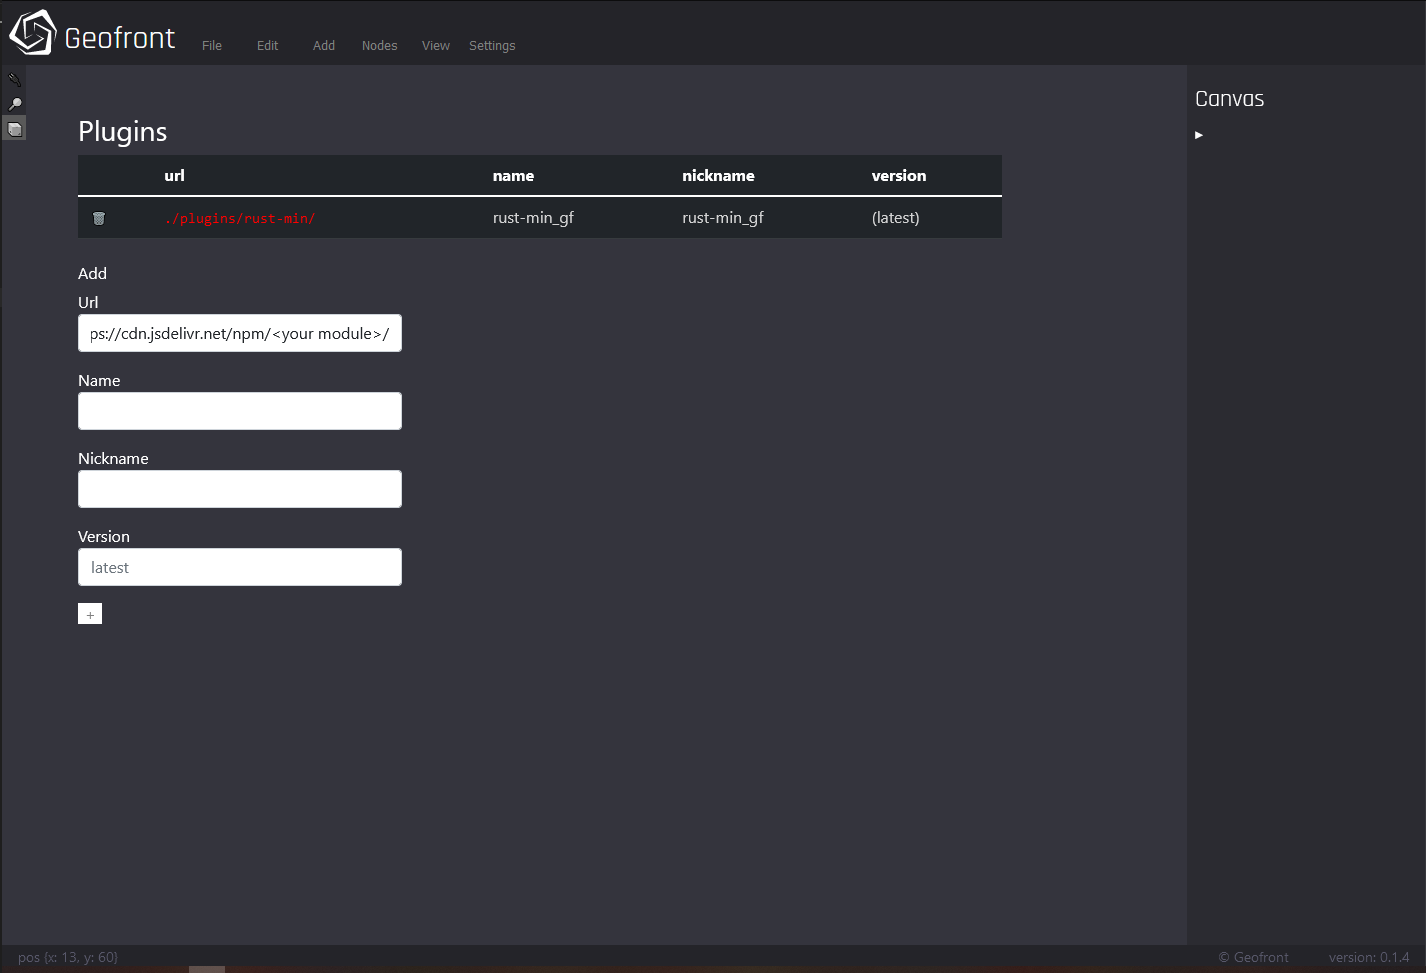
\includegraphics[width=0.50\linewidth]{2.PNG}
  \caption[loading a plugin]{Loading a plugin into Geofront using the \ac{GUI}}
  \label{fig:min-rust-plugin-import}
\end{figure}

\begin{figure}
  \centering
  \begin{subfigure}[b]{0.45\linewidth}
    \graphicspath{{../../assets/images/6.1.1/}}
    \centering
    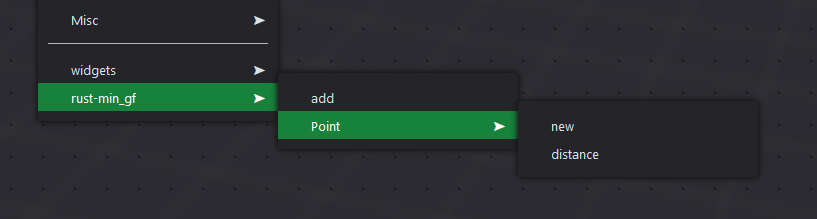
\includegraphics[width=\linewidth]{7.PNG}
    \caption{}\label{fig:rust-plugin-on-canvas:1}
  \end{subfigure}%
  \qquad %-- that adds some space between th 2 figures
  \begin{subfigure}[b]{0.45\linewidth}
    \graphicspath{{../../assets/images/6.1.1/}}
    \centering
    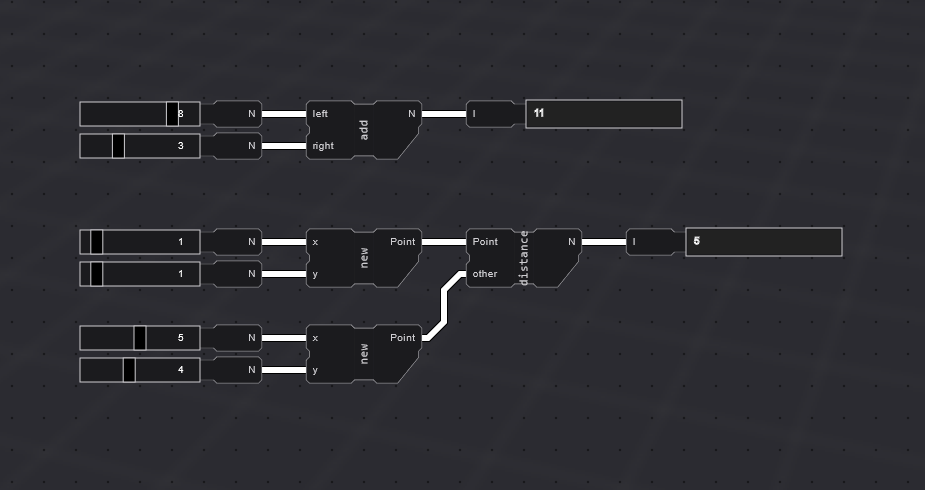
\includegraphics[width=\linewidth]{6.PNG}
    \caption{}\label{fig:rust-plugin-on-canvas:2}
  \end{subfigure}%
  \caption[minimal rust geofront plugin: usage]{Usage On the canvas}
  \label{fig:rust-plugin-on-canvas}
\end{figure}

\subsection{Rust: startin plugin}

Loading the \m{startin} library also occurred as expected.
startin already offered a wasm-ready library, this could directly be loaded into Geofront. 
However, the API exposed by this library used a non-functional style, making it hard to properly use the library on a VPL canvas. 
This is why a custom plugin library still had to be created, in which functions like '\m{new\_from\_vec}' were added to support functional usage. 

Other than that, all steps performed by the minimal Rust plugin could be made with this project as well, as shown in \reffig{fig:startin-plugin}. 
This also showcases the usage of optional, additional bindings:
A series of functions are given definition, which together flag the Triangulation type as 'Renderable'. 
This way, a variable of type 'Triangulation' can be viewed in 3D by clicking on it.

\begin{figure}
  \centering
  \begin{subfigure}[b]{0.90\linewidth}
    \graphicspath{{../../assets/images/6.1.2}}
    \centering
    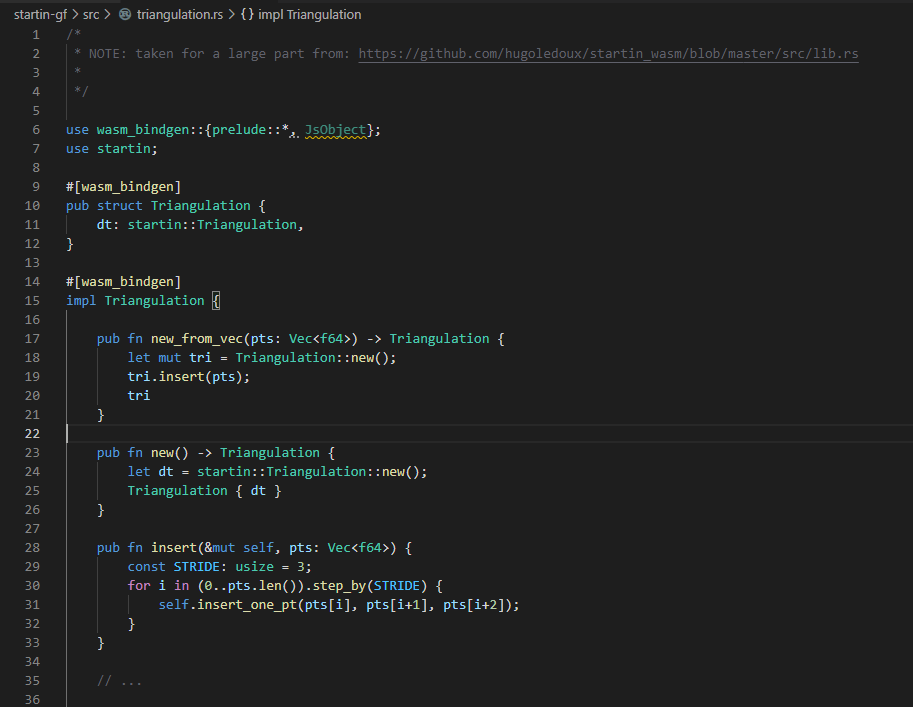
\includegraphics[width=\linewidth]{1.PNG}
  \end{subfigure}%
  \\ 
  \begin{subfigure}[b]{0.90\linewidth}
    \graphicspath{{../../assets/images/6.1.2}}
    \centering
    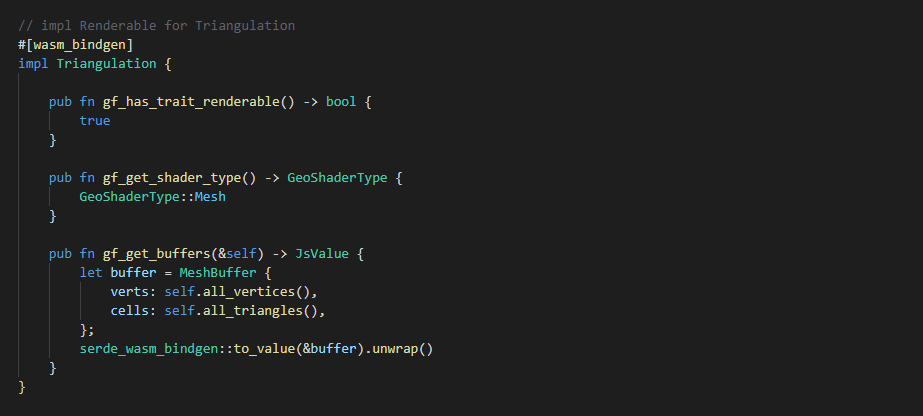
\includegraphics[width=\linewidth]{5.PNG}
  \end{subfigure}%
  \\
  \begin{subfigure}[b]{0.90\linewidth}
    \graphicspath{{../../assets/images/6.1.2}}
    \centering
    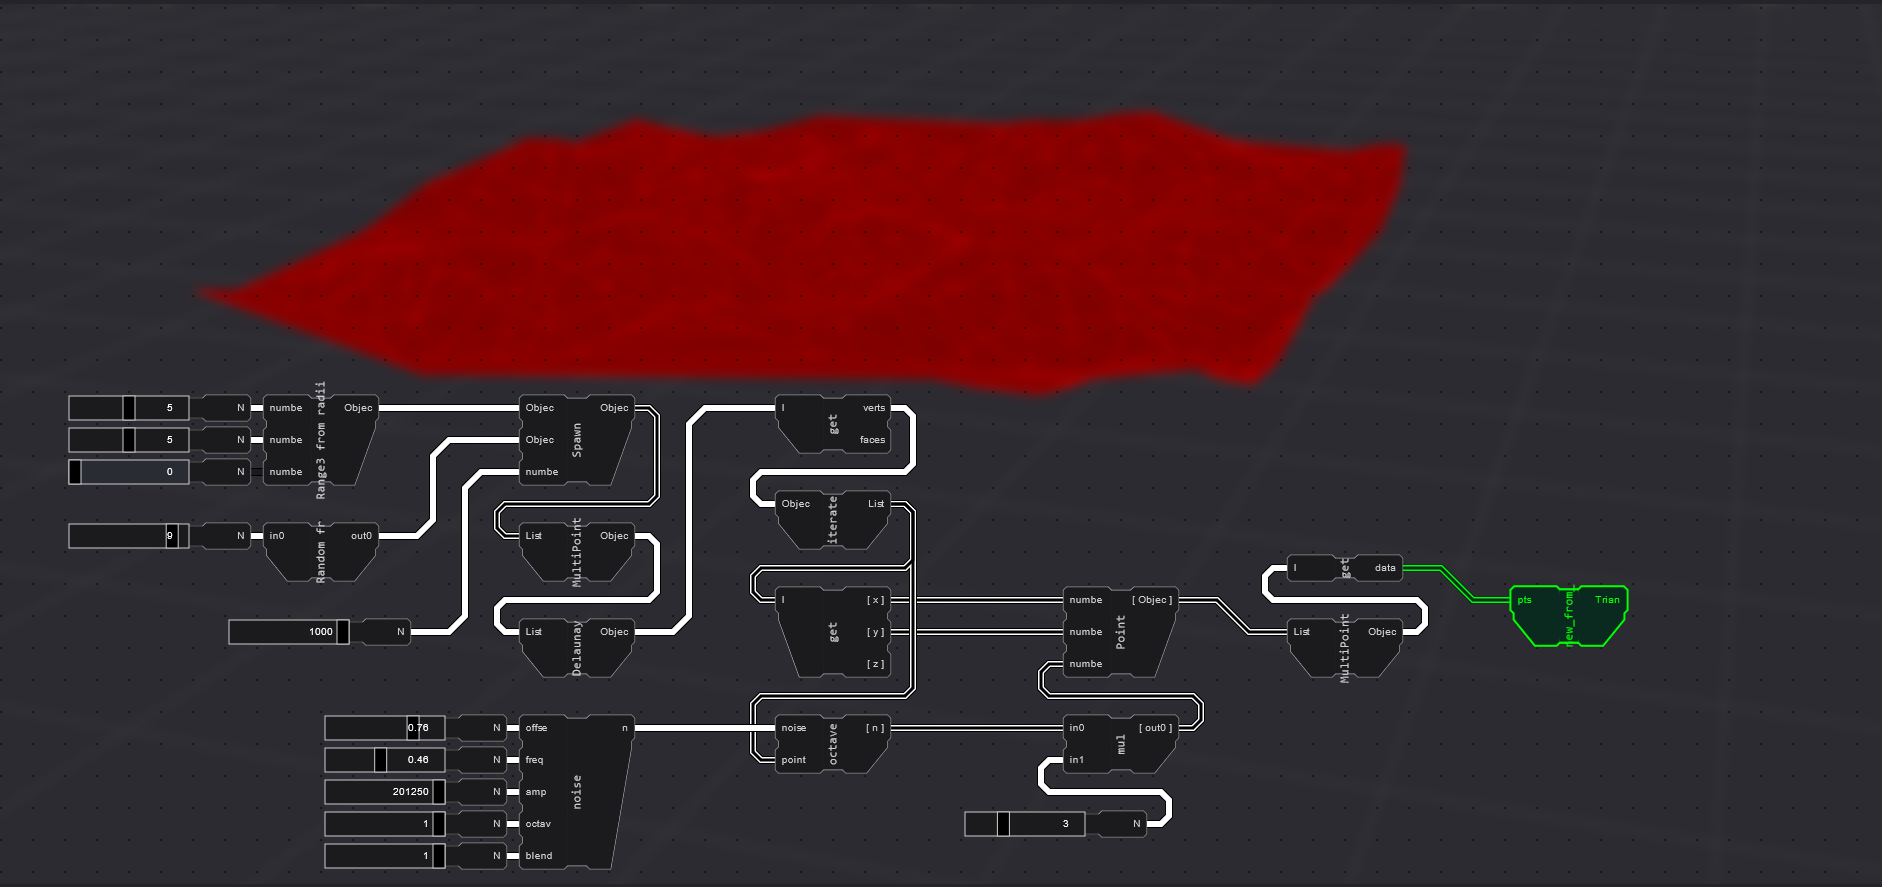
\includegraphics[width=\linewidth]{2.PNG}
  \end{subfigure}%
  \caption[Types of \ac{vpl}s]{Startin, loaded as plugin within Geofront}%
  \label{fig:startin-plugin}
  \end{figure}

\subsection{C++: Minimal plugin}  

\begin{figure}
\centering
\begin{code}
#include <emscripten/bind.h>
#include <cmath>

using namespace emscripten;

float add(float left, float right) {
    return left + right;
}

class Point {
public:
    double x;
    double y;

    Point(double x, double y) :
        x(x),
        y(y) {}

    double distance(Point other) {
        return std::pow(
            std::pow(x - other.x, 2) + std::pow(y - other.y, 2), 
            0.5);
    }
};

EMSCRIPTEN_BINDINGS(cpp_min) {
    function("add", &add);
    class_<Point>("Point")
        .constructor<double, double>()
        .function("distance", &Point::distance)
        .property("x", &Point::x)
        .property("y", &Point::y);
}
\end{code}
\caption{C++: Minimum WebAssembly example}
\label{fig:minimum-cpp-wasm}
\end{figure}

No unexpected shortcomings were encountered in making a minimal C++ WebAssembly build in Geofront.
It was possible to compile the plugin file to WebAssembly, and to use it in a web demo, but this build was limited in its ability to be automatically interfaced with Geofront.
The web demo itself was also more limited compared to the rust build.

First of all, the construction of the C++ source code itself.
Emscripten's \m{embind} tool uses a macro syntax to flag functions marked for javascript compilation, shown in \reffig{fig:min-cpp-source}. 

While it does work similar to Rusts \m{wasm-bindgen}, cpp macro's do not allow for any pre-compile-time code checking, and can produce hard to decipher error messages. 

Secondly, to compile this file to the right binary with accompanied javascript wrapper, it had to be compiled using the \\ \m{-sMODULARIZE=1} and \m{-sEXPORT\_ES6=1} flags enabled.
Otherwise, the javascript produced uses an import syntax too deviant from regular import statements to have any chance to be interfaced by Geofront. 
It must be noted that emscripten was behind on documentation compared to 'wasm-pack' and the rust-wasm organization \citep{contributors_wasm-pack_2022}. 
it does not offer many examples, or thorough explanations on what many of the compiler flags do or mean \citep{emscripten_organization_emscripten_2022}.
wasm-pack on the other hand offers complete tutorials, a range of starter projects, and elaborate documentation of most of its functionalities. 

Thirdly, the compilation with the right flags enabled resulted in a valid '\m{wasm}' and '\m{js}' file, but not a '\m{d.ts}' file.
Emscripten does not support typescript declaration files, and third-party tooling to add this is only conceptual at this point in time. 
This study was also unable to find any developments indicating development towards Interface Types.
All of this does allow for a working web demo similar to the Rust equivalent, shown in \reffig{fig:min-cpp-demo}. However, the absence of interface types, or the substitute typescript interface types, made automated interfacing with the binary difficult. 

This study did eventually achieve a workaround by using javascript reflection.
By creating a blacklist of all 134 default functions the emscripten javascript wrapper comes with with the aforementioned flags enabled, we can distill the imported module down to the 2 symbols exposed by embind in this case, the \m{add} function and \m{Point} class.
However, by doing this, all function types and the names of all parameters are lost, and can not be loaded into Geofront, which in turn does not allow the resulting Geofront graph to be type safe. 
Another solution would have been to manually declare type definitions as strings in the CPP file or as a typescript file, but was deemed a too manual of a solution to a problem which should be able to be solved programmatically, as 'wasm-pack' did.

with a custom system in place to load embind files, the plugin loader could attempt to load both the js and wasm file. 
It is here were an obstacle was encountered, which could not be solved within the time frame of this study. 
The JavaScript wrapper file dynamically fetches the WebAssembly file. 
This is allowed when importing a javascript library using ES6 module syntax. 
However, this is incompatible with the implementation choices of the Geofront plugin loader. 
To load a plugin dynamically, it fetches and interprets the source files at runtime. 
However, for security reasons, dynamically fetching a wasm file from within these runtime interpretations is not allowed.
The \m{wasm-pack} solution does not have the same problem, for it allows the WebAssembly file to be parsed within its initialization function.
A change within the emscripten javascript wrapper would allow this obstacle to be overcome, but this must be left to subsequent research. 

A final workaround was made to still load the plugin within Geofront (\reffig{fig:min-cpp:workaround}). 
However, this was done by forgoing the concept of a plugin, and by integrating the WebAssembly binary within the source code of Geofront itself.
As this thesis is a study on direct accessibility of any \ac{GIS} library, and not on creating the most feature-rich \ac{GIS} web \ac{VPL} imaginable, this solution was discarded.    
However, it does shows that if one forgoes all design constraints, it is fully possible to run and use C++ libraries in Geofront. 

\begin{figure}
  \graphicspath{{../../assets/images/6.1.3}}
  \centering
  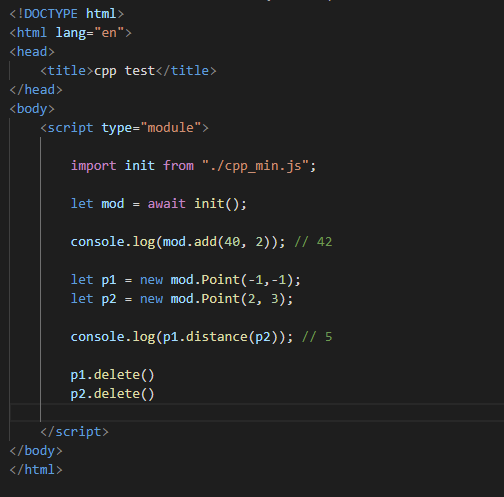
\includegraphics[width=0.50\linewidth]{demo.PNG}
  \caption[loading a plugin]{Cpp-wasm web demo}
  \label{fig:min-cpp-demo}
\end{figure}

\begin{figure}
  \graphicspath{{../../assets/images/6.1.3/}}
  \centering
  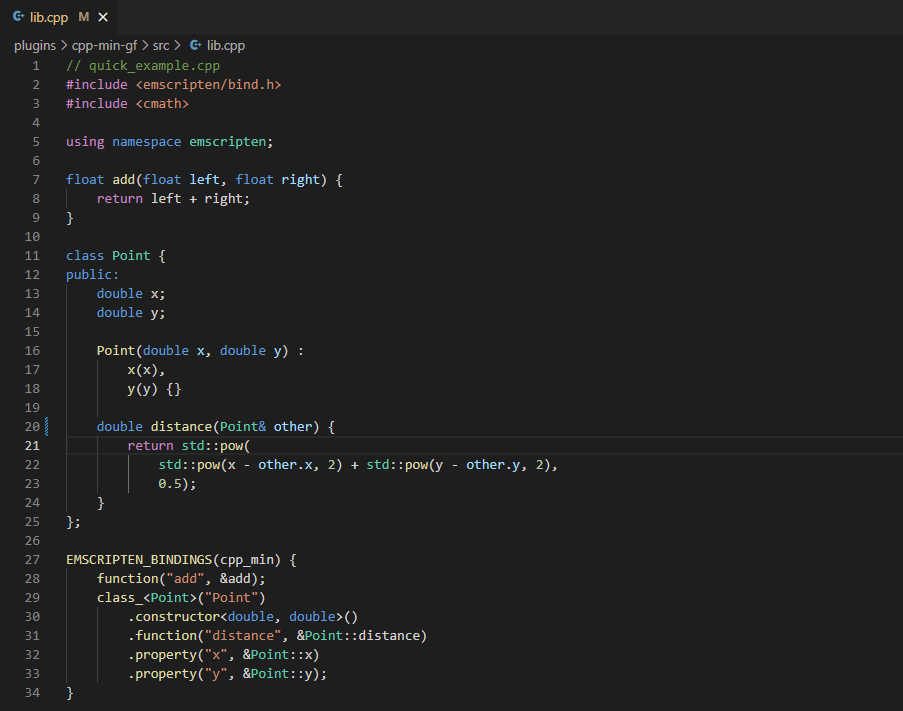
\includegraphics[width=0.50\linewidth]{source.PNG}
  \caption[loading a plugin]{Cpp Plugin Source file}
  \label{fig:min-cpp-source}
\end{figure}

\begin{figure}
  \graphicspath{{../../assets/images/6.1.3/}}
  \centering
  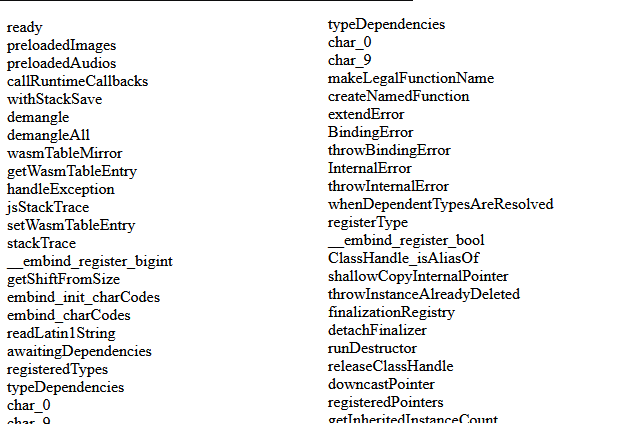
\includegraphics[width=0.50\linewidth]{blacklist.PNG}
  \caption[loading a plugin]{Emscripten JavaScript wrapper blacklist }
  \label{fig:min-cpp-whitelist}
\end{figure}

\begin{figure}
  \graphicspath{{../../assets/images/6.1.3/}}
  \centering
  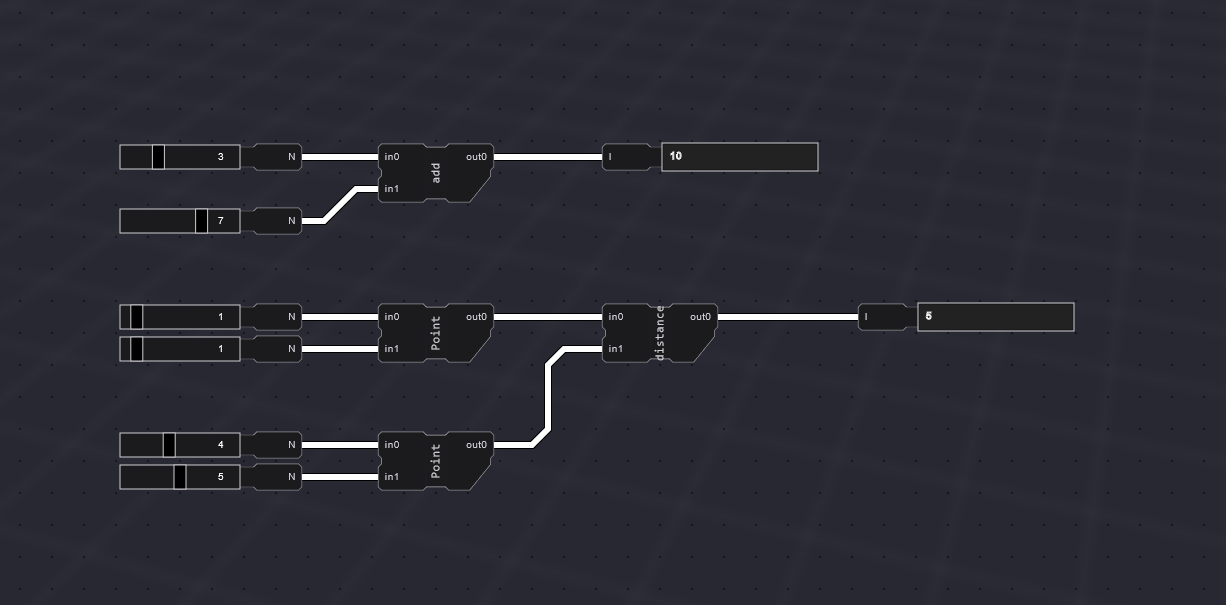
\includegraphics[width=0.50\linewidth]{graph.PNG}
  \caption[loading a plugin]{The result of the workaround: including the C++ binary within the standard library of Geofront}
  \label{fig:min-cpp:workaround}
\end{figure}

\subsection{C++: CGAL plugin}

If the minimum cpp plugin example could not be loaded into Geofront, it will be unsurprising that the entirety of CGAL could also not be compiled into a suitable format ready for VPL consumption.
Several steps towards this goal were made however.

WebAssembly compilation was partially successful.
A web demo was able to utilize the CGAL kernel for basic operations, as can be seen in \reffig{fig:cgal-tryout-2}. 
Additionally, A subsequent web demo can utilize the CGAL TIN to a limited extent (\reffig{fig:cgal-tryout-3}).

However, this demo too could not be fully completed. The major obstacle preventing full usage was making sure all dependencies, like Boost, are compiled together with CGAL.
Legacy makefile build systems complicate this process. 
To get the current demo's working, several dependencies and sub-dependencies had to be manually traversed, their makefiles had to be edited, and the projects had to be re-compiled and copied to different location, to be used by the emscripten compiler exclusively. 
This is an unsustainable workflow, which will complicate development.  

Secondly, building a proper interface to a CGAL functionality, such as a triangulation, was difficult due to combination of CGAL's API together with the restrictions imposed by emscripten, and the functional interface of Geofront. 
As an example, a robust manner of providing CGAL with an array of points was not found.
A single point could be provided, but instantiating a number of of points from within JavaScript turned out to be expensive, so much so that the method had to be deemed unusable. 
Additionally, this is difficult to interface from within Geofront, as this would mean a chain of nodes would have to be created, one for each single point (see \reffig{fig:chain-api}). 

The GDAL.js project was analyzed in an attempt to find a possible solution to handling the great number of dependencies \citep*{dohler_gdal_2022}, and interfacing. 
Regrettably, this project too has resorted to incorporating the source code of GDAL and all its dependencies, and has altered them heavily. 
Interfacing was solved by heavy use of emscripten on the side of javascript, to workaround the limitations regarding parsing vectors and arrays. 
To illustrate, a fragment was taken from the \m{inspect\_geotiff} example, shown in \reffig{fig:gdaljs_ugly}.
Actions like these cannot be directly interfaced from Geofronts visual language.

All these factors together made it so a CGAL plugin could not be presented.
This is not to say that a WebAssembly build of CGAL is not possible, but that many additional steps need to be taken to allow an API which is usable in practice. 
% Emscripten is unable to provide this api in its current state. 
To work around all limitations, a more extensive time frame could have allowed this study to:
\begin{enumerate}
\item Translate CGAL and all dependencies to a WebAssembly-acceptable format 
\item Build a wrapper library on the side of C++, offering a functional interface while remaining compatible with C++, Geofront, and Emscripten's way of interfacing with WebAssembly.  
\item Build a custom importer on the side of Geofront, to provide certain wrappers around emscripten compiled projects.
\end{enumerate}
However, much of this would be simplified if emscripten adopts the features found in \m{wasm\_pack} and \m{wasm\_bindgen}, such as interface types, and support for vectors and arrays without pre-allocation. 

\begin{figure}
  \graphicspath{{../../assets/images/6.1.4/}}
  \centering
  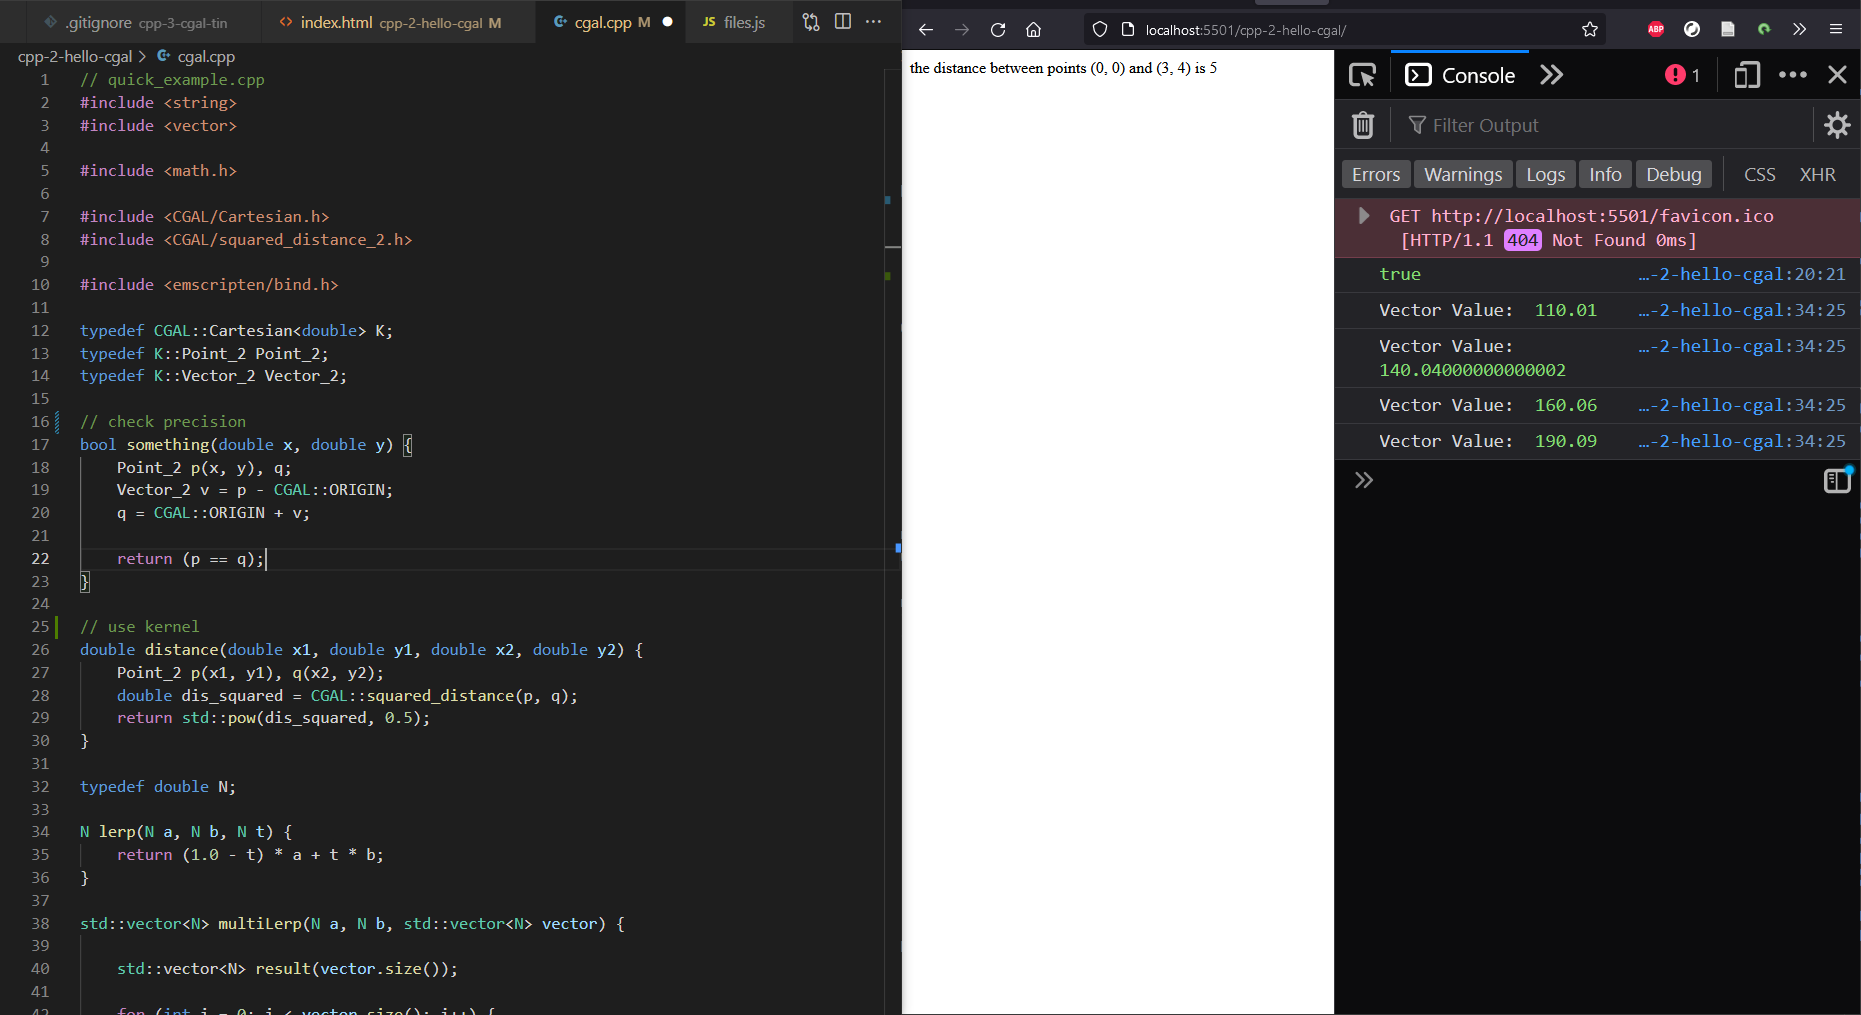
\includegraphics[width=\linewidth]{demo-2.PNG}
  \caption[loading a plugin]{CGAL Kernel Demo}
  \label{fig:cgal-tryout-2}
\end{figure}

\begin{figure}
  \graphicspath{{../../assets/images/6.1.4/}}
  \centering
  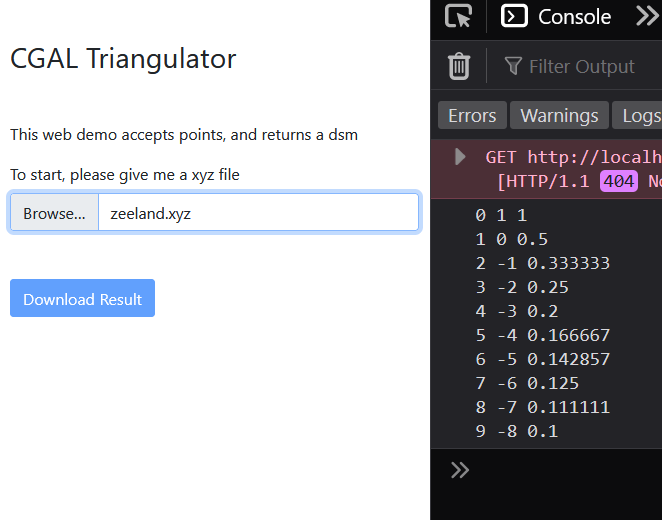
\includegraphics[width=0.50\linewidth]{demo-3.PNG}
  \caption[loading a plugin]{CGAL Triangulation Demo}
  \label{fig:cgal-tryout-3}
\end{figure}

\begin{figure}
  \graphicspath{{../../assets/images/6.1.2/}}
  \centering
  \begin{code}
  // [...]
  
  // This is where things get a bit hairy; the C function follows a common C
  // pattern where an array to
  // store the results is allocated and passed into the function, which 
  // populates the array with the
  // results. Emscripten supports passing arrays to functions, but it always 
  // creates a *copy* of the
  // array, which means that the original JS array remains unchanged, which 
  // isn't what we want in this
  // case. So first, we have to malloc an array inside the Emscripten heap  
  // with the correct size. In this
  // case that is 6 because the GDAL affine transform array has six elements.

  var byteOffset = Module._malloc(6 * Float64Array.BYTES_PER_ELEMENT);
  
  // byteOffset is now a pointer to the start of the double array in Emscripten 
  // heap space
  // GDALGetGeoTransform dumps 6 values into the passed double array.
  
  GDALGetGeoTransform(dataset, byteOffset);
  
  // Module.HEAPF64 provides a view into the Emscripten heap, as an array of 
  // doubles. Therefore, our byte offset
  // from _malloc needs to be converted into a double offset, so we divide it 
  // by the number of bytes per double,
  // and then get a subarray of those six elements off the Emscripten heap.
  
  var geoTransform = Module.HEAPF64.subarray(
      byteOffset/Float64Array.BYTES_PER_ELEMENT,
      byteOffset/Float64Array.BYTES_PER_ELEMENT + 6
  );
  
  // [...]
  \end{code}
  
  \caption[]{A fragment from the \m{inspect\_geotiff} example found in GDAL.js. Source: \citet{dohler_gdal_2022}}
  \label{fig:gdaljs_ugly}
\end{figure}

\begin{figure}
  \graphicspath{{../../assets/images/6.1.2/}}
  \centering
  \includegraphics[width=0.50\linewidth]{chain-API.PNG}
  \caption[]{If only one point can be provided at a time, this would become the API in Geofront for adding three points: A long chain of additions}
  \label{fig:chain-api}
\end{figure}


% The first one has to do with rewriting inputs and outputs to CGAL functionality.
% The most common ways to provide CGAL functions with data, and to retrieve results, is to read and write files. 
% While this can be used on the web, the virtual file system wrappers presented by Emscripten add irregular syntax to the plugin, again compromising any chance it can be loaded into Geofront.
% So, a way is needed to present CGAL with data directly from javascript or other wasm binaries, without reading or writing files. 
% Initial tests were performed by parsing input data as a string buffer, which could then be 'read' like a file by CGAL.

% Additionally, many scientifically oriented C++ libraries like CGAL make extensive use of meta programming and template programming, paradigms which do not translate well to an environment outside of C++. 

\subsection{Comparison}

A couple of additional comparisons between the four WebAssembly projects mentioned above were made, both in terms of the file size of the compiler artifacts, as well as the performance of specifically the interoperability between WebAssembly and javascript. 
These are the results:

\subsubsection*{Size}

\begin{figure}
  \graphicspath{{../../assets/plots/rust-cpp-performance/}}
  \centering
  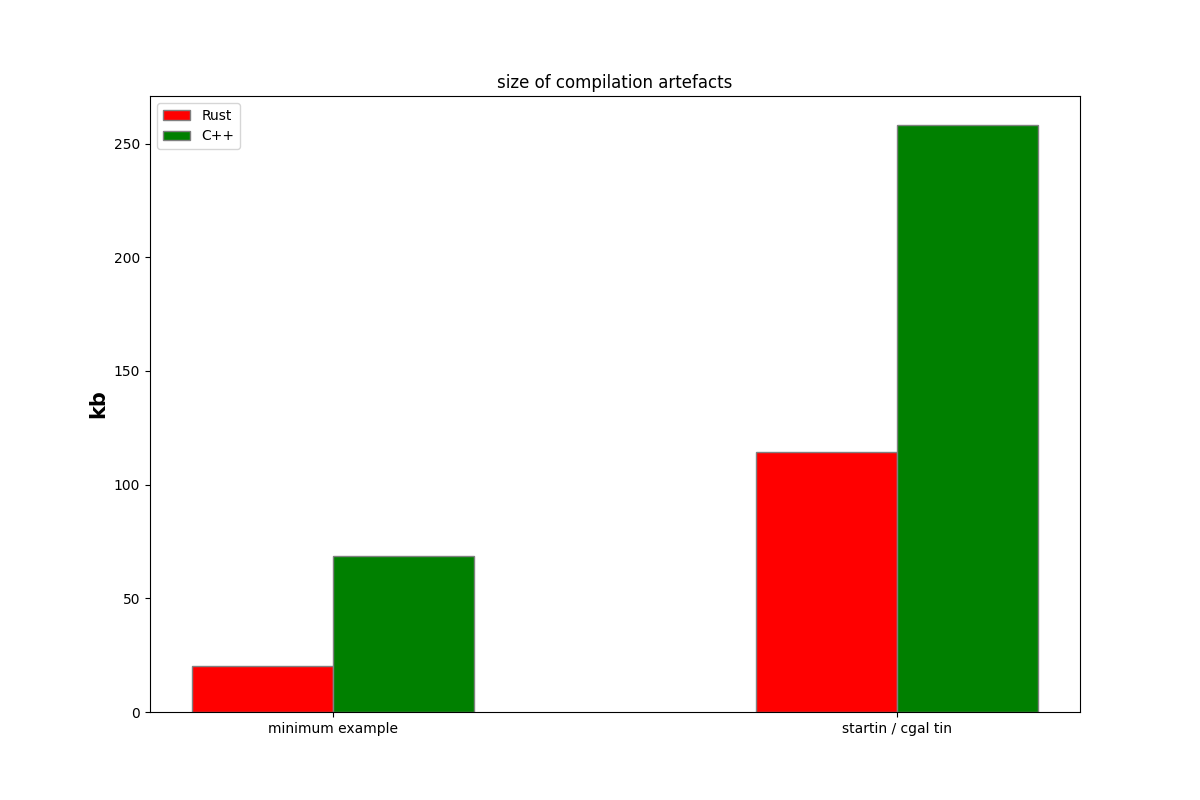
\includegraphics[width=\linewidth]{figure.png}
  \caption[]{Combined size of all compiler artifacts produced by either wasm-pack or emscripten}
  \label{fig:rust-cpp-compilation}
\end{figure}

\reffig{fig:rust-cpp-compilation} shows how the minimum C++ plugin compiles to a binary of 68424 bytes. 
Compared to the Rust build of 20140 bytes, This is around 3.4 times more. 
The CGAL TIN test compiled to 257994 bytes, and compared to startin's 114263 bytes, is around 2.3 times more heavy.

The wasm-pack artifacts include the typescript header files, and both its typescript and javascript file were not optimized for size.
Emscripten does not produce a typescript file, and compressed its javascript file maximally. 

All of these facts combined make it safe to say that the emscripten wrappers are significantly heavier.

This study speculates this difference could be because emscripten's primary use-case is compiling complete applications. 
This requires a more heavy wrapper, offering features like file servers. 
When compiling sizable C++ applications, the overhead of this wrapper can be marginalized.
However, apparently, emscripten is not able to distinguish between full applications, and small, granular use-cases like this one, and must include the 'full emscripten runtime' in all cases.

\subsubsection*{Performance}

\begin{figure}
  \graphicspath{{../../assets/plots/rust-cpp-compilation-size/}}
  \centering
  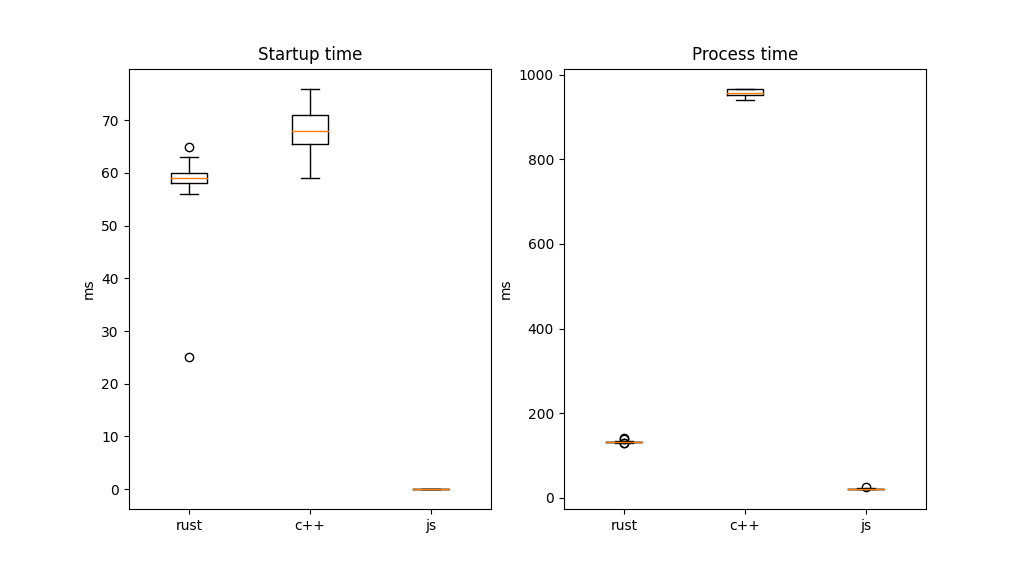
\includegraphics[width=\linewidth]{figure.png}
  \caption[]{A benchmark using three comparable demo's handling points, given 100.000 iterations}
  \label{fig:rust-cpp-performance}
\end{figure}

To test the performance of \ac{wasm} - javascript interaction, the minimum C++ and Rust plugins were again used. 
This makes for a good comparison, since both projects deliver the exact same functionality from the point of view of javascript.  
A pure javascript version was added however, to add a base comparison.
The web pages used for these tests are presented in \reffig{fig:perf-benchmark}.

% fig:rust-cpp-performance

% The performance benchmarks. 
% These benchmarks primarily test how performant the \\ javascript - WebAssembly interactions are. 


% TODO APPENDIX?
The results are can be seen in in \reffig{fig:rust-cpp-performance}.
These results show the emscripten wrapper is not as performant as the wasm-pack solution.
From experimentation, performance hit could be narrowed down to the initialization step of the 'Point' classes. 

These results may suggest two phenomena:
One, just like the artifact size comparison, this difference could be because emscripten is written from the point of view of a C++ application, and use case does not require custom javascript - C++ interoperability. 
A full application seldom needs access to specific javascript processes the way this demo does. 
such an application only needs to address javascript through emscripten own interface, which could be more performant. 

And two, the C++ builds may be suffering from 'legacy burden', as described by \citet{ammann_maplibre-rs_2022}. 
The emscripten solution needs to take more edge cases into account, has more complicated dependencies, and software compiled using emscripten must be more heterogenous than a younger language like Rust.
This all could lead to a significant performance hit.

\begin{figure}
  \centering
  \begin{subfigure}[b]{0.32\linewidth}
    \graphicspath{{../../assets/images/6.1.5/}}
    \centering
    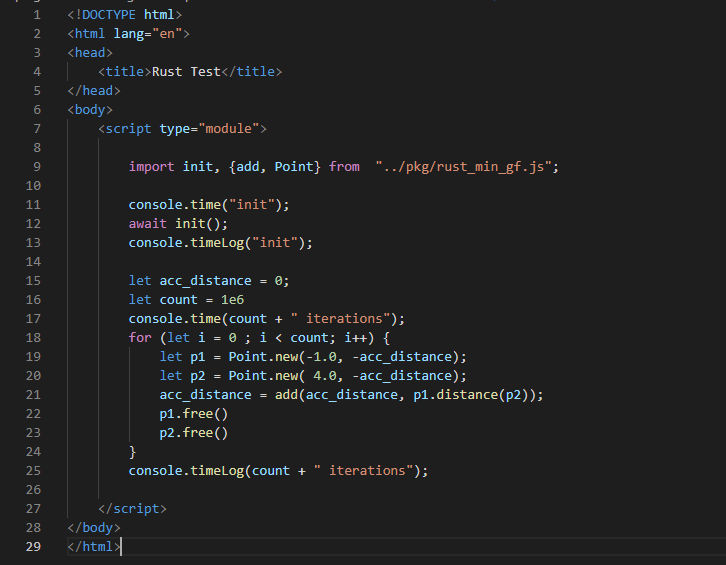
\includegraphics[width=\linewidth]{rust.PNG}
    \caption{}
  \end{subfigure}%
  \qquad %-- that adds some space between th 2 figures
  \begin{subfigure}[b]{0.32\linewidth}
    \graphicspath{{../../assets/images/6.1.5/}}
    \centering
    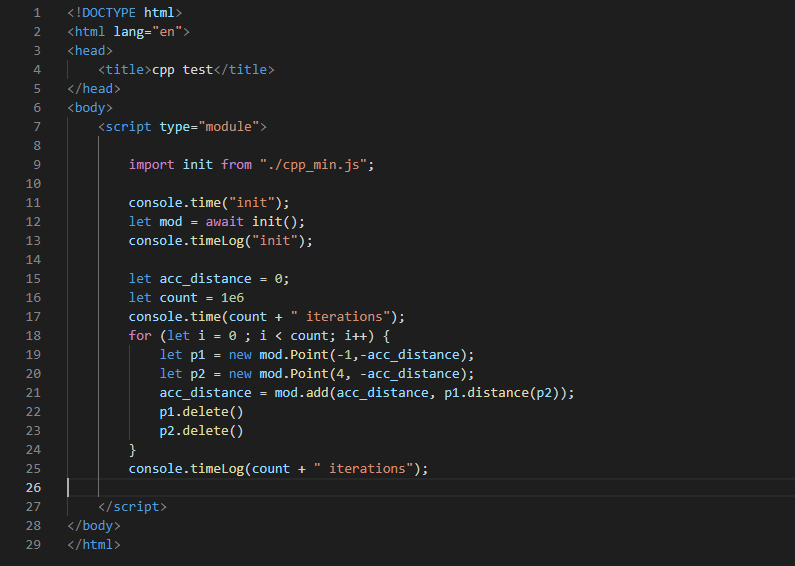
\includegraphics[width=\linewidth]{cpp.PNG}
    \caption{}
  \end{subfigure}%
  \qquad
  \begin{subfigure}[b]{0.32\linewidth}
    \graphicspath{{../../assets/images/6.1.5/}}
    \centering
    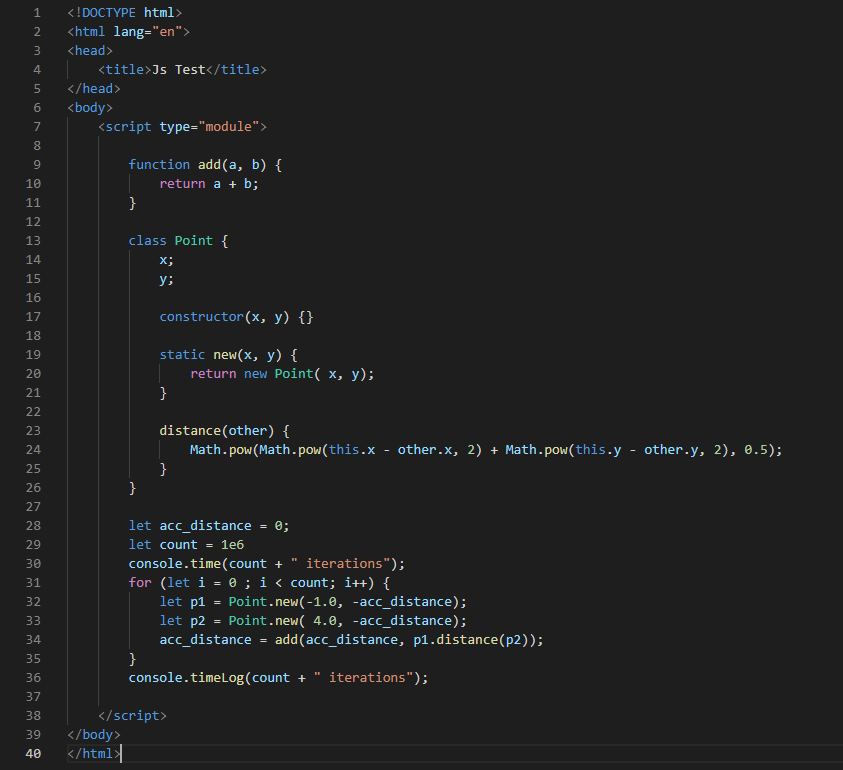
\includegraphics[width=\linewidth]{js.PNG}
    \caption{}
  \end{subfigure}%
  \caption[benchmark]{Rust vs C++ vs js performance benchmarks}
  \label{fig:perf-benchmark}
\end{figure}


\section{Demo applications}
\label{sec:testing:demo}
% - Show a demo
This section demonstrates the extend to which Geofront is able to perform the main role it set out to fulfill: 
Accessing functions from low level \ac{GIS} libraries from within a web VPL, and subjecting these functions to to interactive elements, so that these functions may be used in different ways by end users.

Two related demo applications are presented, both featuring the \m{startin} library covered in \refsec{sec:testing:compilation}.
The following two sections demonstrate the achieved functionality, and implications of said functionality. 
the last section presents the limitations encountered during the writing and usage of these demo's.

\subsection{Demo One: Perlin noise \& startin}

\graphicspath{{../../assets/images/6/demo/}}

\begin{figure}
  \centering
  \begin{subfigure}[b]{0.90\linewidth}
    \centering
    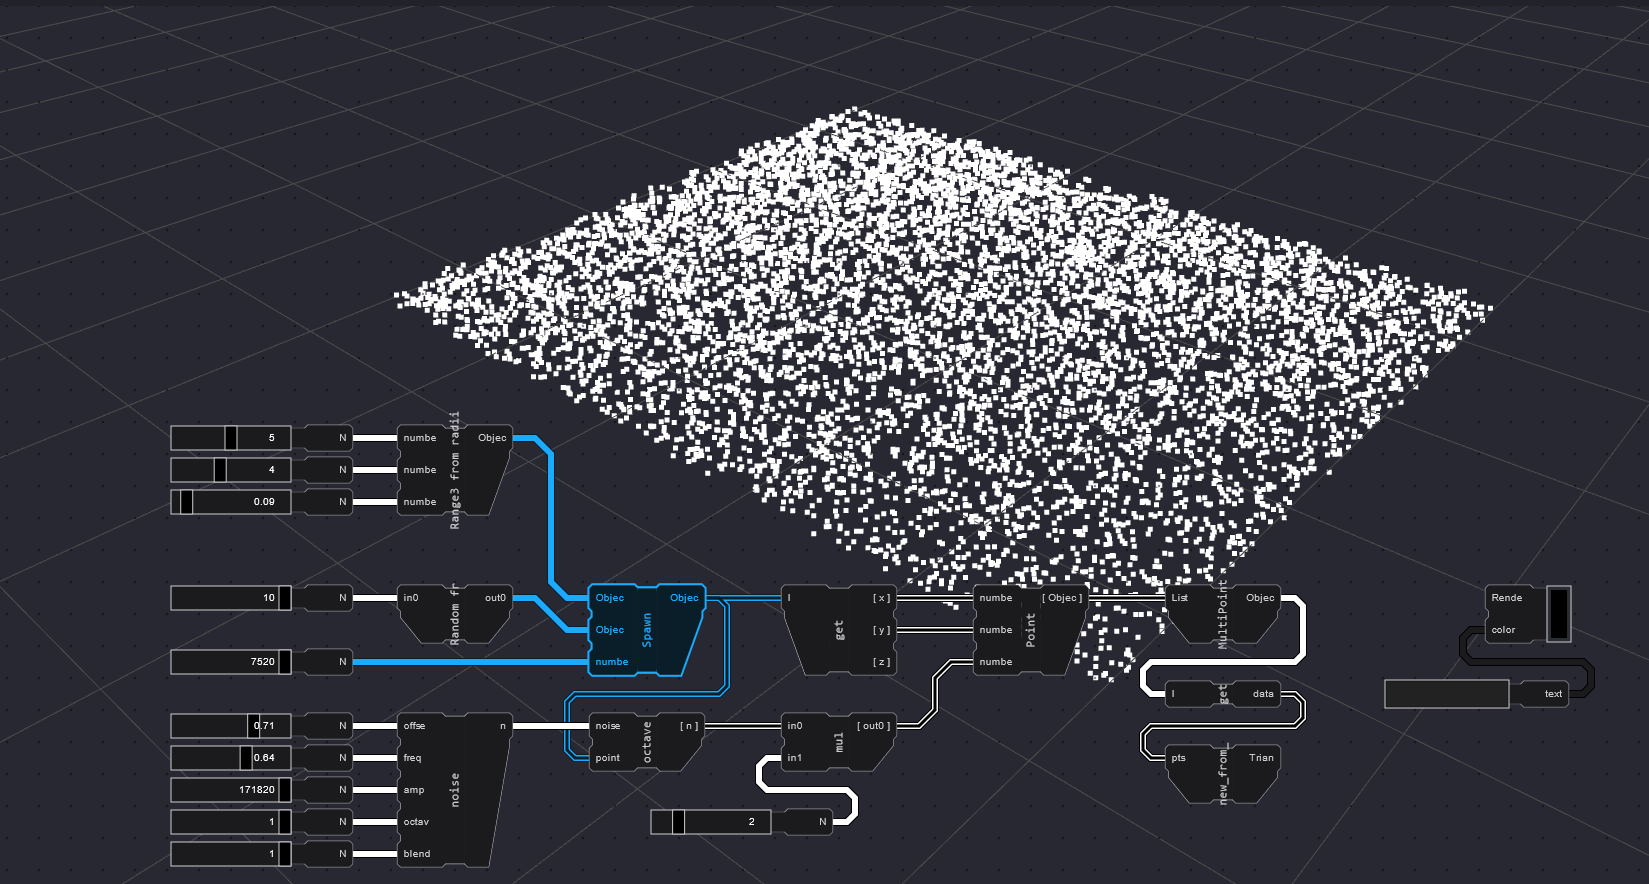
\includegraphics[width=\linewidth]{products-1.PNG}
    \caption{}\label{fig:in-between-products:a}
  \end{subfigure}%
  \\ 
  \begin{subfigure}[b]{0.90\linewidth}
    \centering
    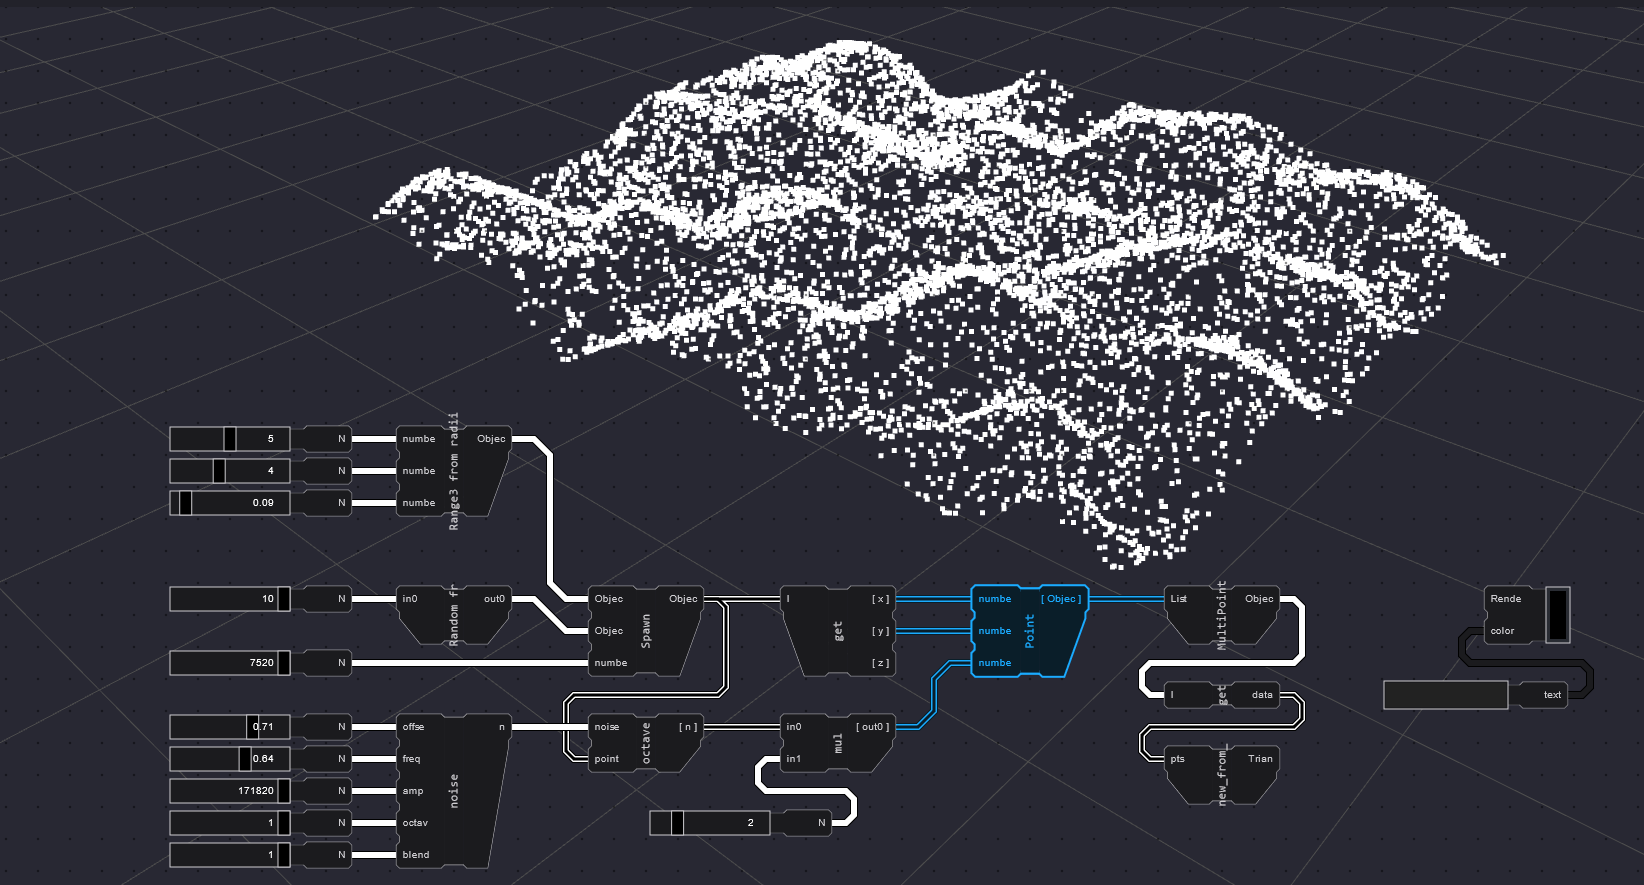
\includegraphics[width=\linewidth]{products-2.PNG}
    \caption{}\label{fig:in-between-products:b}
  \end{subfigure}%
  \\
  \begin{subfigure}[b]{0.90\linewidth}
    \centering
    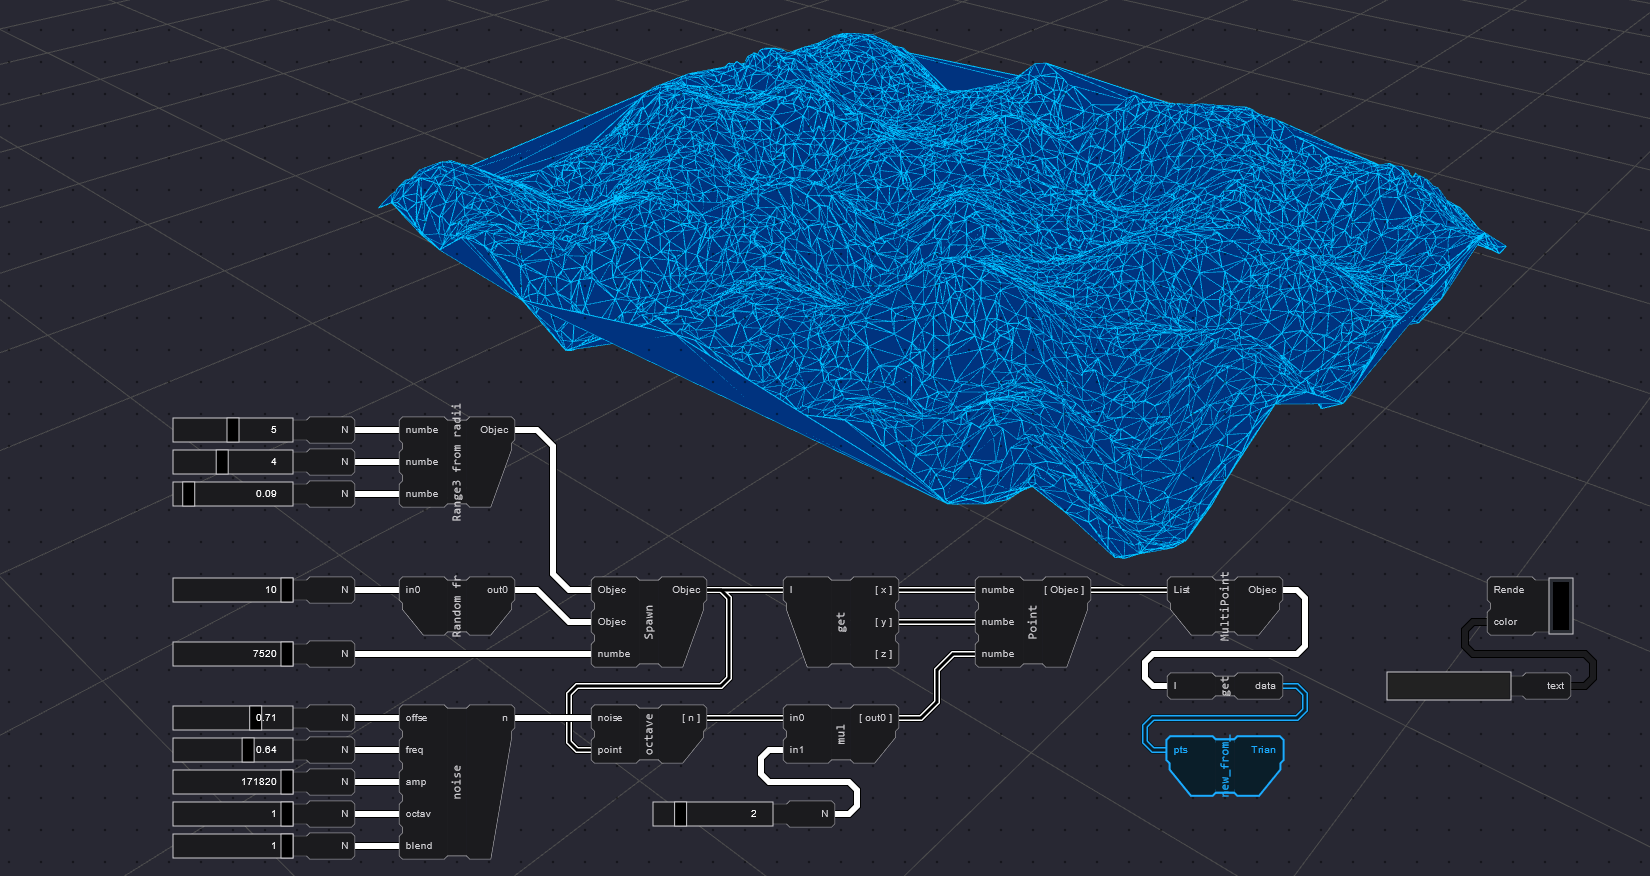
\includegraphics[width=\linewidth]{products-3.PNG}
    \caption{}\label{fig:in-between-products:c}
  \end{subfigure}%
  \caption[]{Visual inspection of in-between products}%
  \label{fig:in-between-products}
\end{figure}

\begin{figure}
  \centering
  \begin{subfigure}[b]{0.90\linewidth}
    \centering
    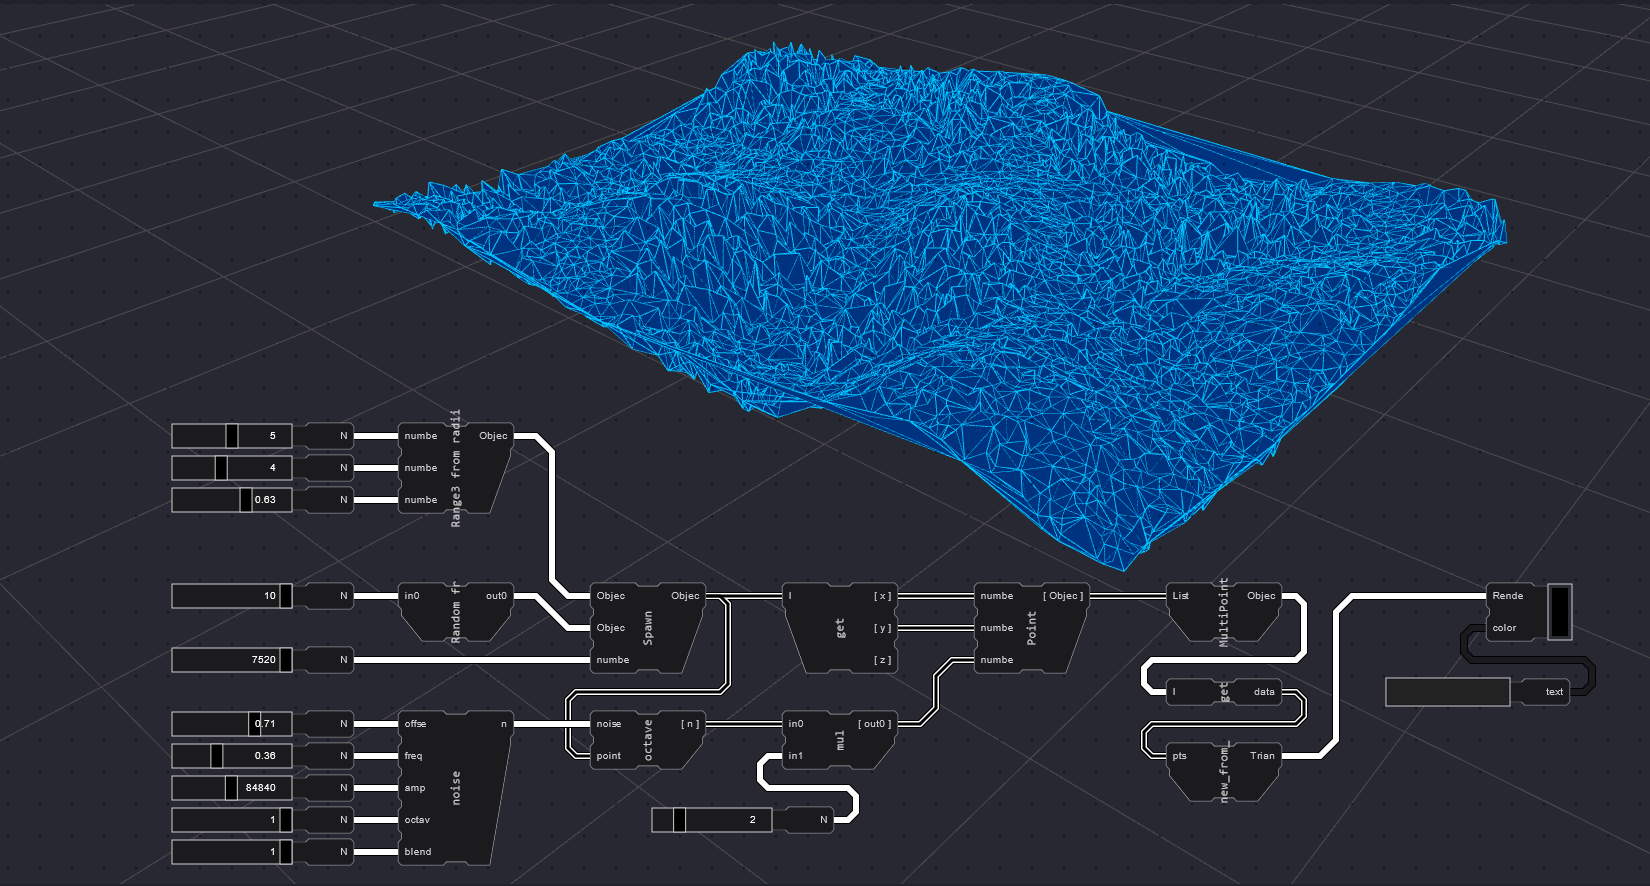
\includegraphics[width=\linewidth]{explore-1.PNG}
  \end{subfigure}%
  \\ 
  \begin{subfigure}[b]{0.90\linewidth}
    \centering
    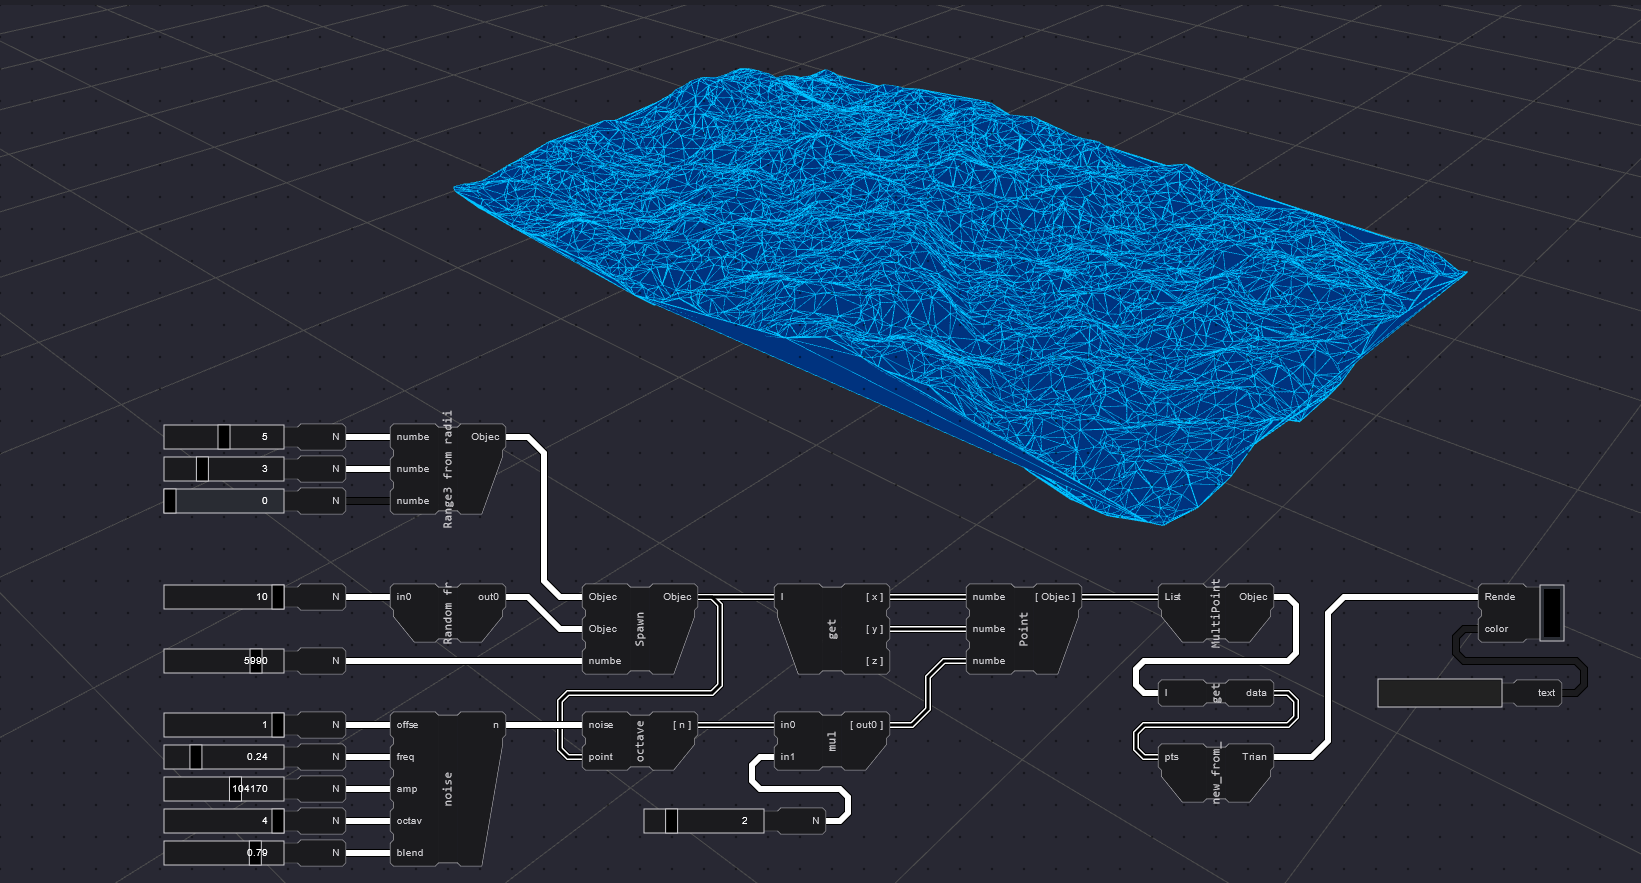
\includegraphics[width=\linewidth]{explore-2.PNG}
  \end{subfigure}%
  \\
  \begin{subfigure}[b]{0.90\linewidth}
    \centering
    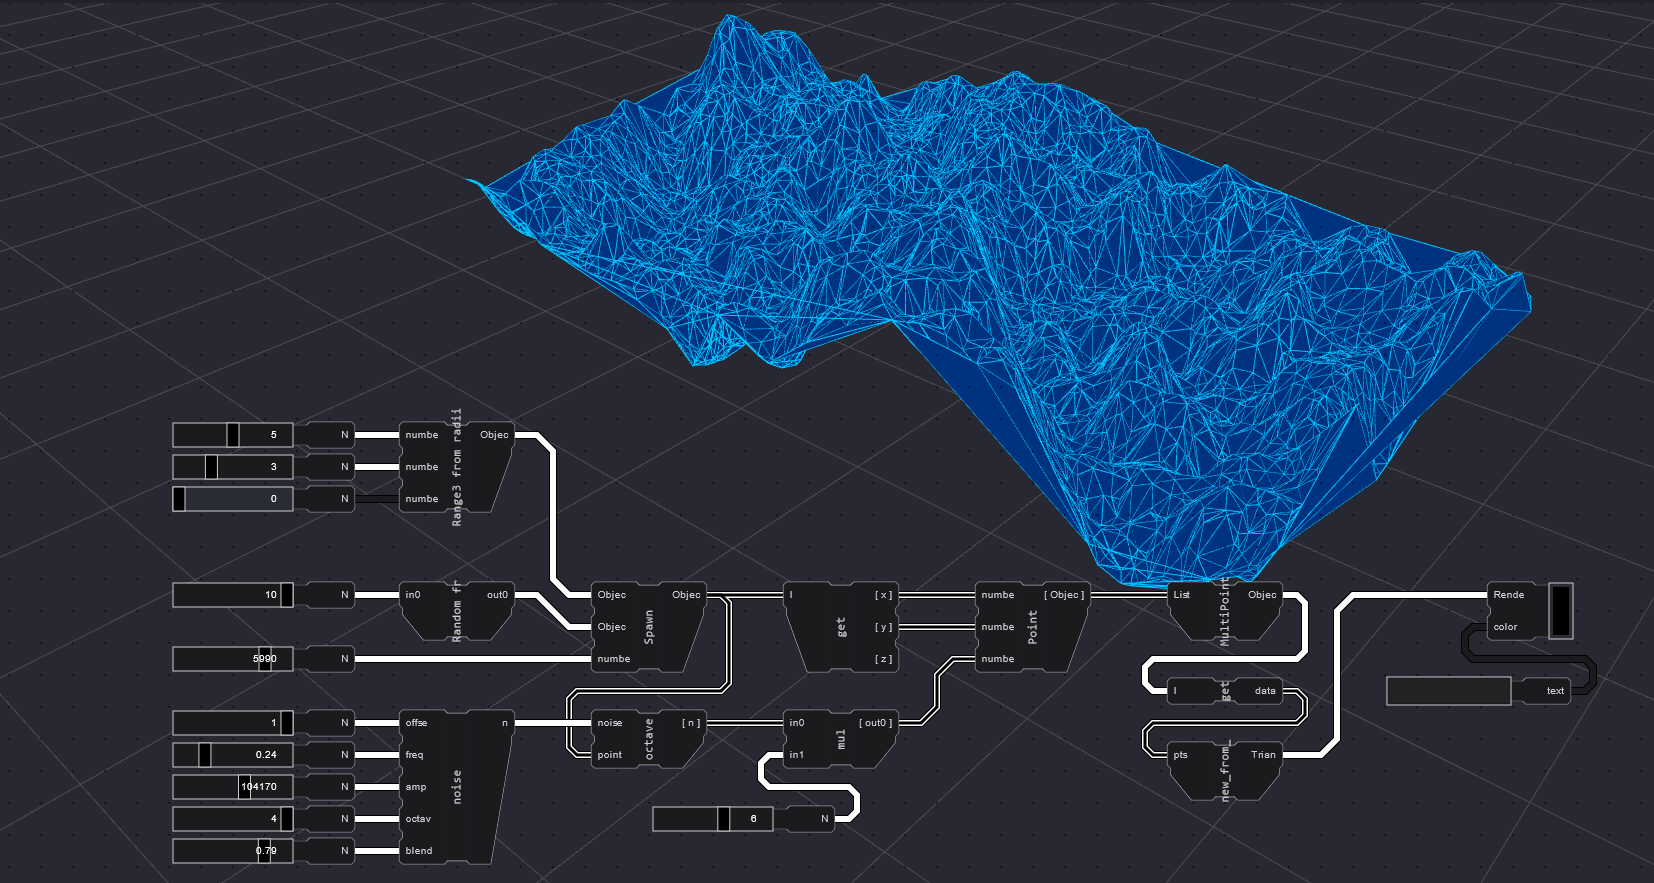
\includegraphics[width=\linewidth]{explore-3.PNG}
  \end{subfigure}%
  \caption[]{Exploration of the effects of different parameters}%
  \label{fig:parametrization}
\end{figure}


The first demo application demonstrate Geofronts core ability to connect a native library to an arbitrary UI. 
In this hypothetical scenario, we wish to discover how the \m{startin} triangulation reacts to various terrains by subjecting it to different point samples: Smooth samples, noisy samples, homogenous or heterogenous point distribution.

In reality, the \m{startin} triangulation serves as a normal 2.5D delaunay triangulation, so we do not expect to see any strange behavior, but one can imagine other terrain extraction and generalization algorithms where a test like this would grant valuable insights.  
An example of such an algorithm would be a plane fitting algorithm using RANSAC. or least squares adjustment of a polynomial surface.

A test setup is made to generate various terrains using Perlin Noise \citep{perlin_improved_2002}, so that different landscapes could be simulated.
This setup not provide a way to generate different sample densities, but it will serve for the purposes of this demo.

The resulting geometry pipeline can be seen in \reffig{fig:in-between-products}. 
A UI is created by using multiple slider widget as inputs numbers.
These numbers are used to create a bounding box area, which is subsequently filled with a random distribution of points (\reffig{fig:in-between-products:a}).
The input sliders are also used to construct a noise field, which is sampled using these points. These noise values are used as the heights of the points (\reffig{fig:in-between-products:b}).
Lastly, these points are used as input for the \ac{TIN} (\reffig{fig:in-between-products:c}).

Multiple observations can be made from this demo:
Firstly, note how the various visualizations of these in-between products could be inspected by selecting the corresponding operation (\reffig{fig:in-between-products}). 
Secondly, observe how by connecting \m{startin} to this arbitrary \ac{GUI}, the behavior of the library can now be explored with different parameters (\reffig{fig:parametrization}).
Thirdly, recall that this sequence can be altered in real time, without any software alterations. 
These functionalities in conjunction are all indicators that Geofront can indeed be used to explore the capabilities and quality of native \ac{GIS} libraries.

\subsection{Demo Two: DTM \& DSM extraction}

\begin{figure}
  \centering
  \begin{subfigure}[b]{0.90\linewidth}
    \centering
    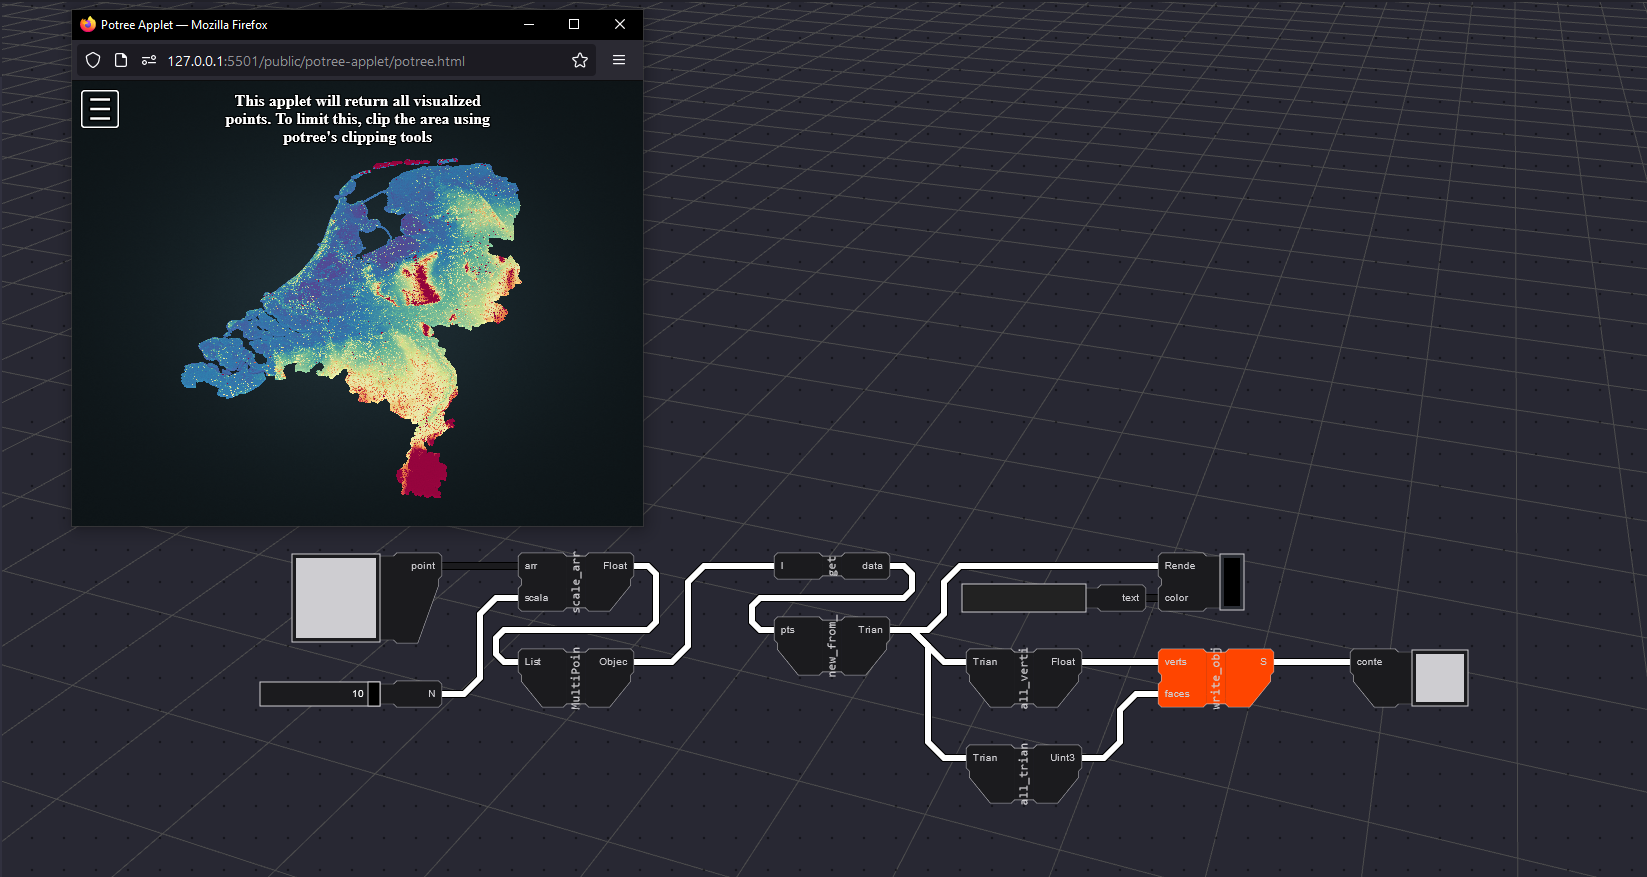
\includegraphics[width=\linewidth]{potree-1.PNG}
  \end{subfigure}%
  \caption[]{DSM and DTM extraction using Potree within Geofront}%
  \label{fig:potree-overview}
\end{figure}

\begin{figure}
  \centering
  \begin{subfigure}[b]{0.90\linewidth}
    \centering
    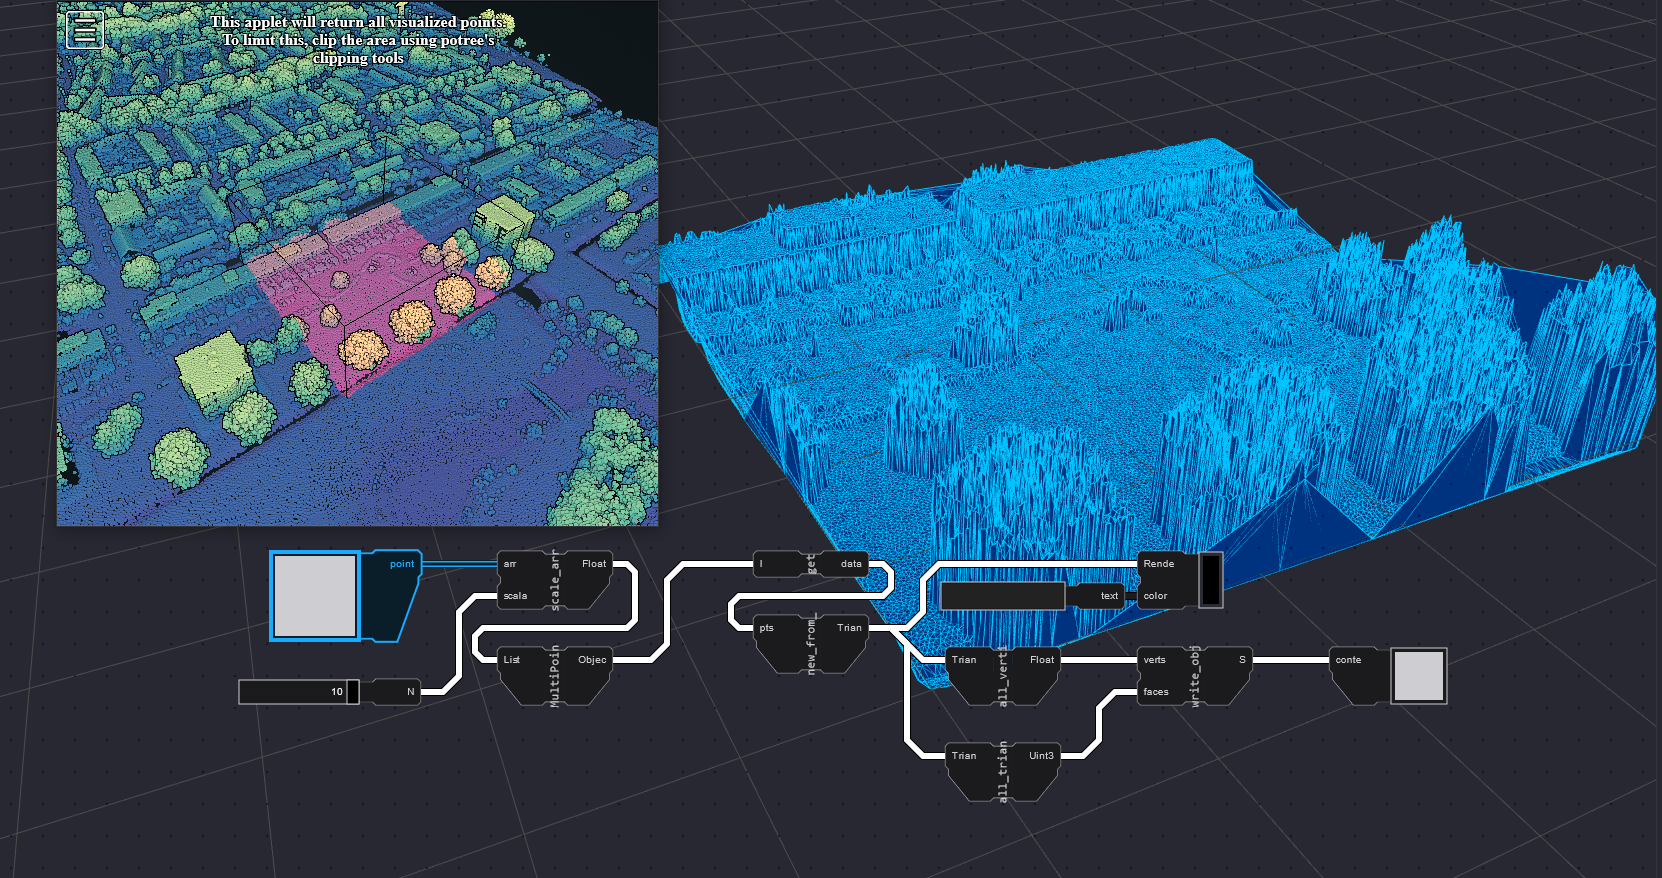
\includegraphics[width=\linewidth]{potree-2.PNG}
    \caption{}\label{fig:potree:a}
  \end{subfigure}%
  \\
  \begin{subfigure}[b]{0.90\linewidth}
    \centering
    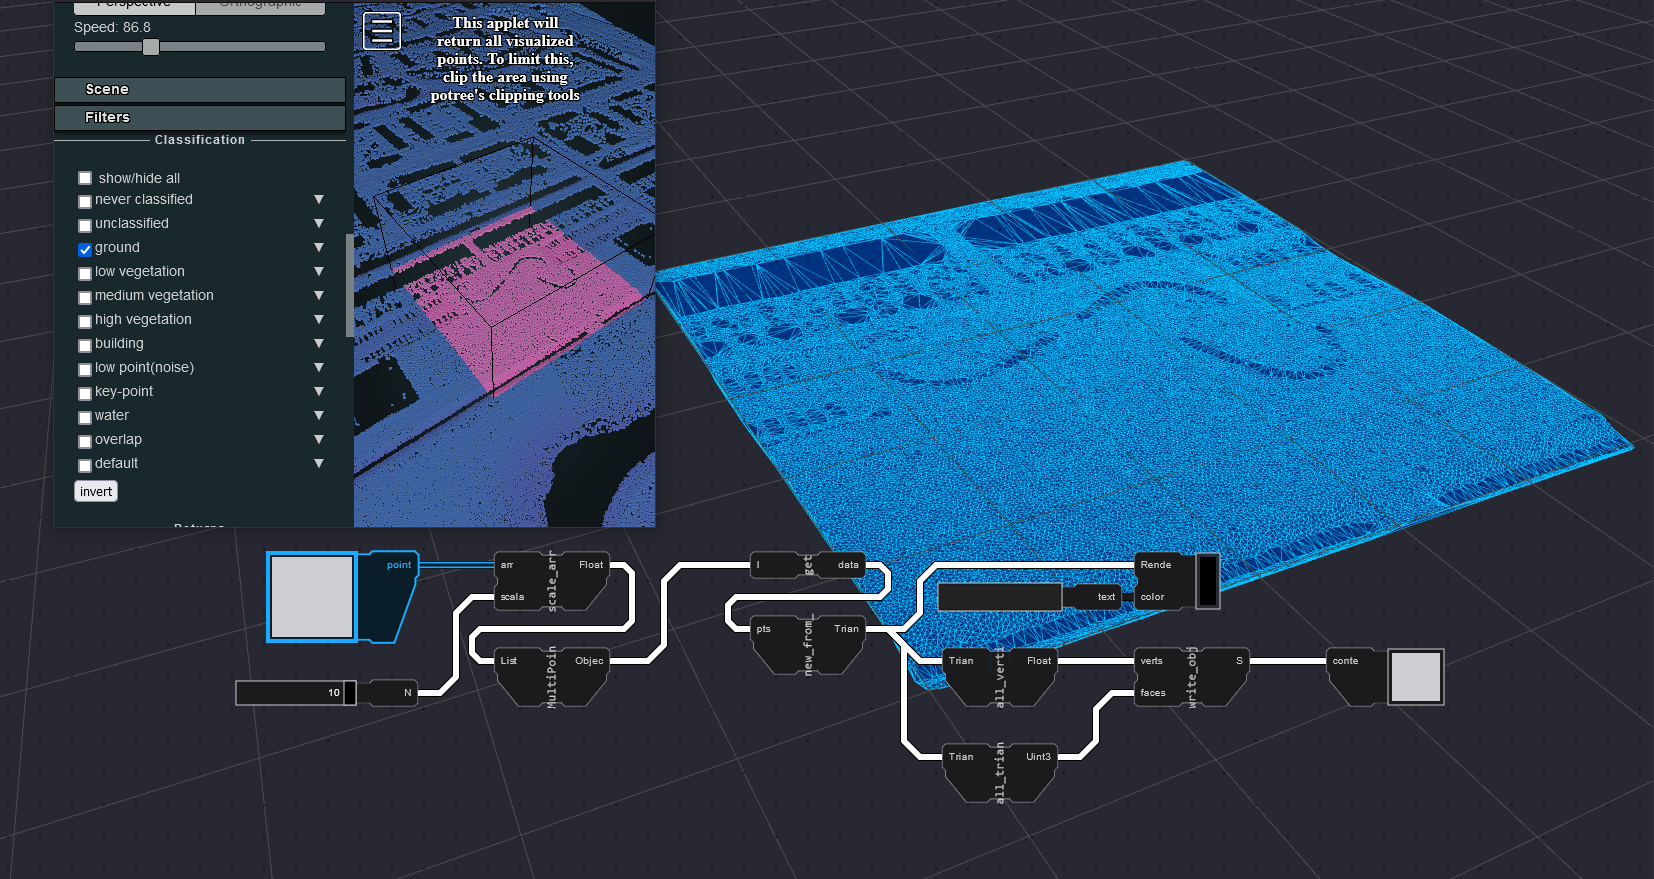
\includegraphics[width=\linewidth]{potree-4.PNG}
    \caption{}\label{fig:potree:b}
  \end{subfigure}%
  \\
  \begin{subfigure}[b]{0.90\linewidth}
    \centering
    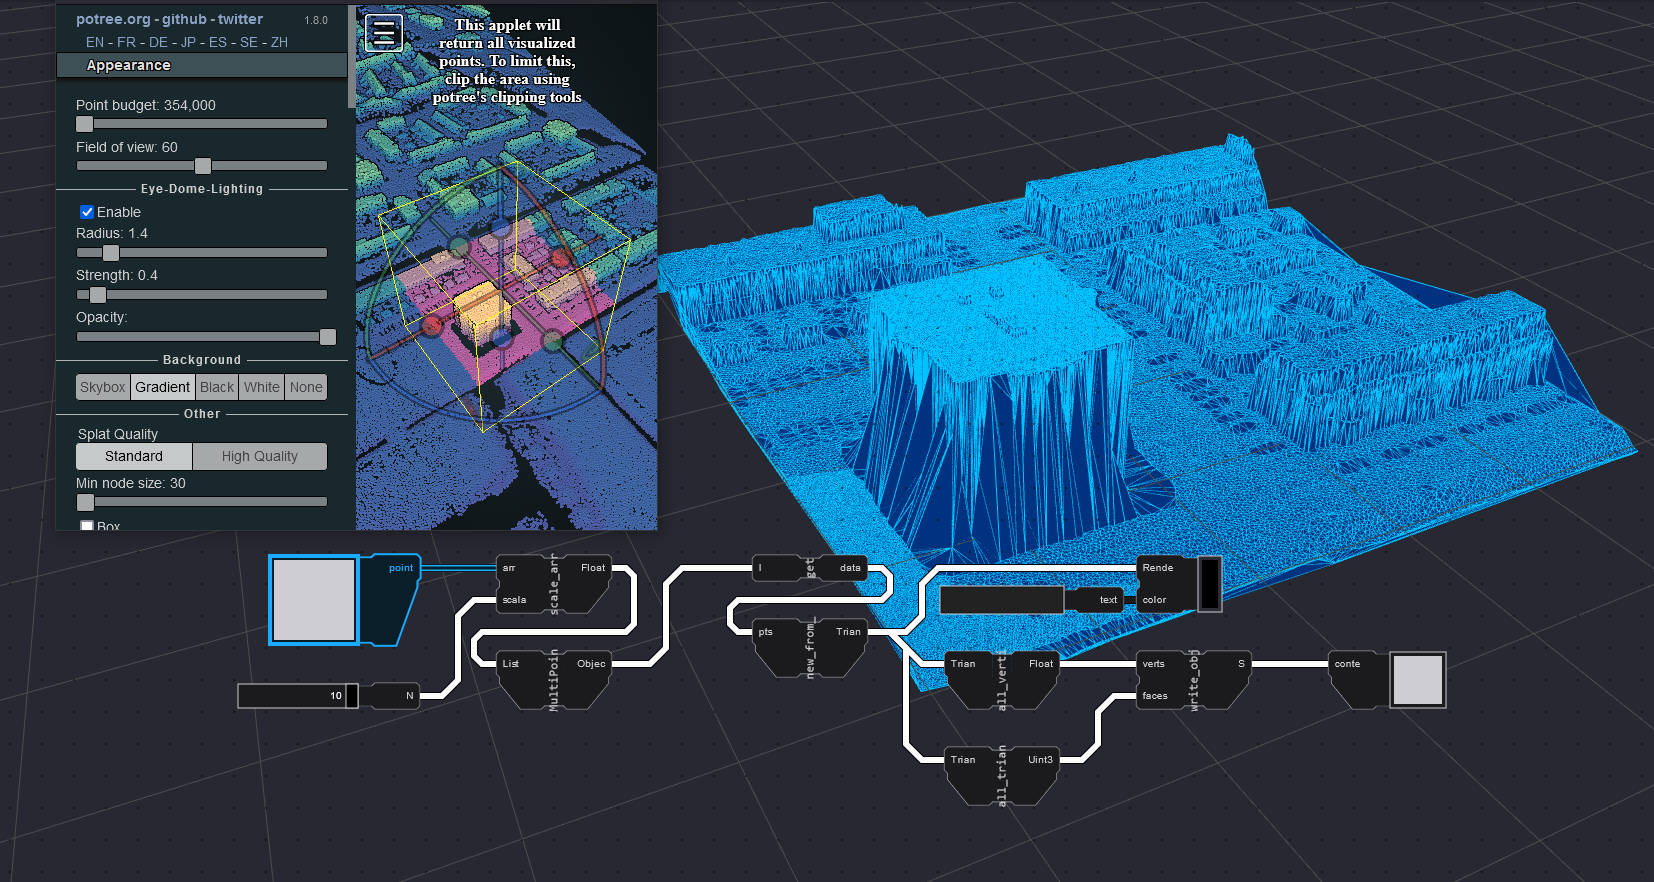
\includegraphics[width=\linewidth]{potree-5.PNG}
    \caption{}\label{fig:potree:c}
  \end{subfigure}%
  \\
  \caption[]{Options when using Potree within Geofront}%
  \label{fig:potree}
\end{figure}

\begin{figure}
  \begin{subfigure}[b]{0.90\linewidth}
    \centering
    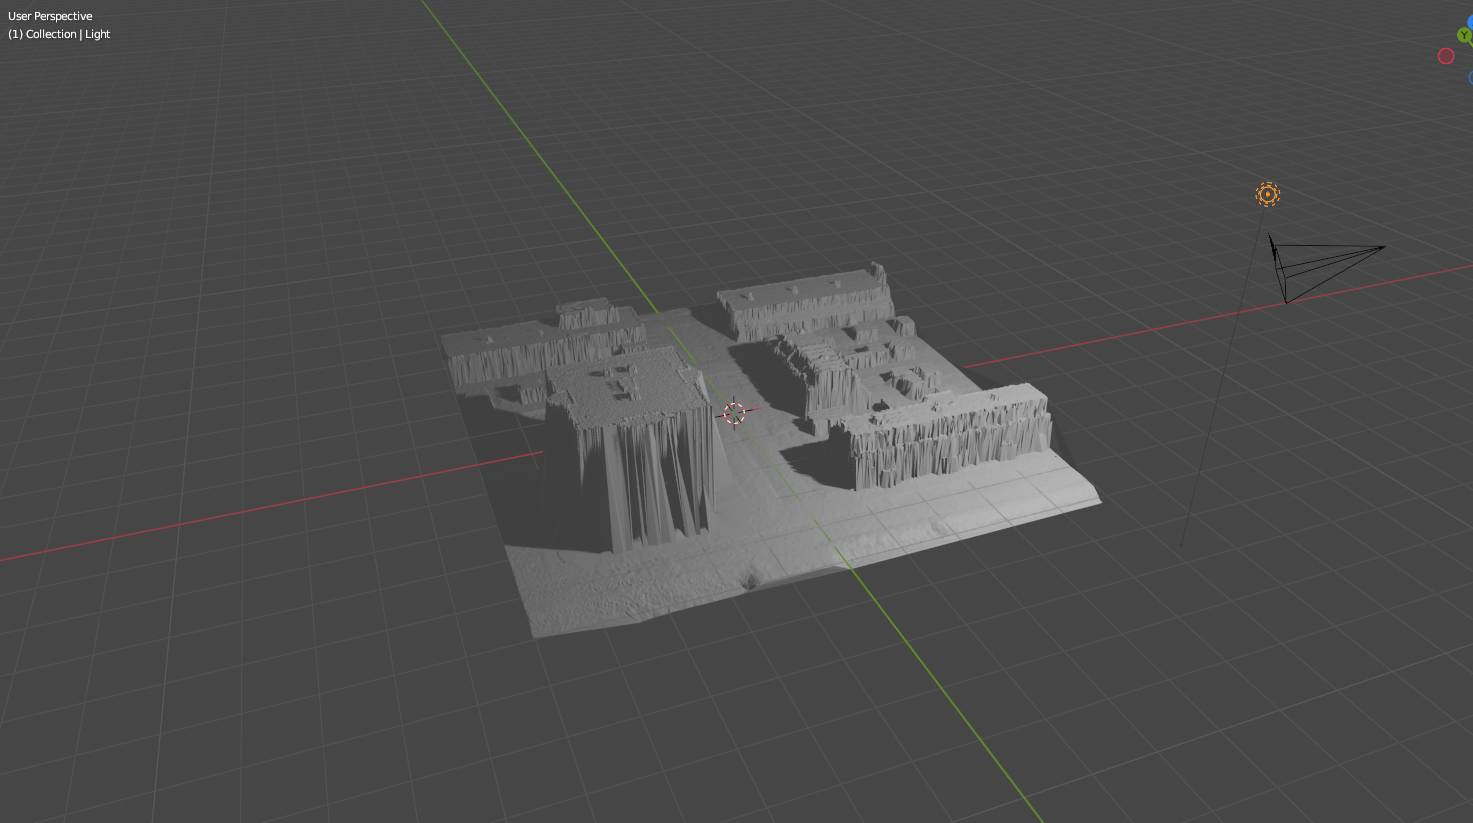
\includegraphics[width=\linewidth]{potree-7.PNG}
  \end{subfigure}%
  \caption{Resulting obj mesh, extracted from the Potree demo}
  \label{fig:potree-result}
\end{figure}

Geofront was meant not only to be used to examine and visualize native libraries, but also to directly utilize them to fulfill real applications.
This second application demonstrates the extend to which this is possible. 

The hypothetical scenario used for this demo, is a situation in which a small scale \ac{DTM} is required from a point cloud. 
One could imagine a \ac{DSM} or \ac{DTM} of a construction site, required for creating an accurate render of a buildings surroundings. 

the above \m{startin} demo is used as a starting point. 
This time, however, a \ac{TIN} will be generated from a real point cloud, instead of a simulated one, and will be converted to a \m{.obj} file, so that the DTM / DSM might be used in a different process. 

The resulting pipeline can be seen in \reffig{fig:potree-overview}. 
Central to this pipeline is the 'Potree applet', found at the start of the pipeline. This is a special type of \ac{UI} widget, which can be used to open a new browser window, running a second application.
This application was created as part of this study, and uses the Potree viewer \citep*{schutz_potree_2022}. 
It can be used independently, but by opening it from within Geofront, a connection between the two applications can be established. 
It allows Geofront to request a pointcloud, by pointing to a publicly hosted, potree-converted dataset. 
The same connection allows Geofront to request parts of this pointcloud, so that a sub section can be used in the Geofront pipeline. 
To query a specific subset, the Potree viewer itself can be used to:
\begin{itemize}[-]
  \item Filter the density of the pointcloud to a desired LOD.
  \item Filter the pointcloud to a certain bounding box or polygon.
  \item Filter the pointcloud based on classifications, to create either: 
  \subitem a DSM using all samples (\reffig{fig:potree:a}),
  \subitem a DTM with only terrain (\reffig{fig:potree:b}), or
  \subitem a DSM with only buildings (\reffig{fig:potree:c}).
\end{itemize}

The pointcloud subset is then loaded into the Geofront pipeline, after it can be used as input for any loaded plugin. 
In this case, the points are inserted to the \m{startin} triangulator, after which the resulting mesh is converted to an \m{.obj} string, and made available for download using a 'save file' widget, so it could be used in a render (\reffig{fig:potree-result}).


Multiple observations can be made based on this demo.
First, notice again how all steps mentioned correspond to the nodes of the pipeline. 
None of these steps are final. 
A different application could be created at runtime, by for example, adding a \m{laz} writer component to save the resulting subset as a point cloud itself, or by using a component to perform a solar potential analysis. 
This application strongly suggests that Geofront can indeed be used to directly utilize native libraries as part of a "real" use-case.
Additionally, it demonstrates that Geofront allows not only composability between libraries, but also between libraries and full-scale, existing applications.

\subsection{Limitations}

Based on the above demo's, the following limitations in utilization were encountered: 
\begin{itemize}
  \item \textbf{Limited STD}: The standard operations and widgets present in geofront are limited. 
  examples of these are scaling a vector, filtering lists, or getting the highest point from a set.
  Additionally, standard \ac{GIS} functionalities, such as reprojections, are also not possible. 
  Currently, plugin libraries add some of these basic functions as a workaround.    

  \item \textbf{Types not interoperable}: While the type system of Geofront is extensive and supports complex aspects such as generics, no clear design is present for interoperating between internal Geofront types, such as a Geofront Mesh, and a foreign type, such as \m{startin}s triangulation. 
  The method used in the above demo's involves breaking down a type into a basic javascript data formats, and using that as an interoperable model. 
  However, this relies on unsustainable parsers which use hardcoded strings, reflection, and "blind thrust".

  \item \textbf{Limited visualization}: Currently, the application is only able to visualize a small number of data types, like points, lines, and meshes. Geofront's source code will have to be altered to support a library using images, for example.
  Another visualization shortcoming is that meshes currently cannot support over 65.535 vertices. 
  
  \item \textbf{Limited performance}: The geofront runtime is not offloaded to a different thread, due to a difficulty of integrating web workers with the logic of the VPL. 
  This means that heavy calculations performed on the canvas will freeze up the \ac{GUI} of the application. 
  % which is not reasonable.  
 
\end{itemize} 

% - Show a bit of performance of said demo


\section{Feature Comparison}
\label{sec:testing:features}

In Table \ref{table:features}, Geofront is compared against the most similar \ac{VPL}s mentioned in \refsec{sec:related-geovpl}.
This comparison was done using the features described in \refsec{sec:method:tests:features}.

Based on this comparison, the implementation of the proposed method appears to indeed provide a unique set of features, not found in comparable visual languages. 
It offers relatively extensive plugin support compared to other VPLs, it is web based, and offers a range of \ac{GUI} nodes. 
Moreover, it is unique in its ability to accept third party Plugins written in different types of languages, and in the fact that it allows custom types within those plugins. 

Geofront's drawback is that it offers no GIS nodes by default, and relies on third party plugins to provide these aspects. 
It can also not yet be regarded as scalable. 
Despite certain design decisions which might aid scalability, no native runtime exist yet which can run a Geofront script in a headless, GUI-less manner.

\begin{table}[h]
\centering
\footnotesize{
\begin{tabular}{
||p{2.8cm}|l|l|l|l|l||}
\hline
& \emph{Grasshopper} & \emph{Blender} & \emph{Mobius} & \emph{Geoflow}    & \emph{Geofront}   \\
\hline
Plugin support    & \textbf{Yes}  & No*    & No     & \textbf{Yes} & \textbf{Yes} \\
Plugin language   & C\#  & -    & -     & C++ & Rust/Js/Ts** \\
Plugin types      & Partially & No      & No     & Unknown    & \textbf{Yes} \\
Headless runtime  & No          & No      & No               & \textbf{Yes} & No         \\
Web based         & No          & No      & \textbf{Yes}     & No           & \textbf{Yes} \\
Base GIS Nodes    & No          & No      & \textbf{Yes}     & \textbf{Yes} & No \\
GUI nodes         & \textbf{Yes} & \textbf{Yes}      & No     & No          & \textbf{Yes} \\
\hline
\end{tabular}
}
\\
--- \\
\footnotesize{* Not without altering the source code of Blender itself \\}
\footnotesize{** theoretically, any language can  be used. 
Practically, only Rust, JavasScript and TypeScript result in valid plugins. \\}

\caption{Feature comparison of relevant VPLs}
\label{table:features}
\end{table}

\subsection{Plugin comparison}

An additional comparison was made between the VPLs which accept third party plugins.
Specifically, the different ways in which a new node has to be registered in Geoflow, Grasshopper, and Geofront are regarded next to each other.

\subsubsection{Grasshopper}

Grasshopper offers an object-oriented approach of registering new nodes: (\reffig{fig:boilerplate:grasshopper}).
A derived class has to be created and configured to represent an addition operation in this case.
While this does lead to a verbose setup, this also makes it so metadata can be included alongside the 'function', as can be seen in the constructor: A name, nickname, and description can be provided.

\begin{figure}
\centering
\begin{code}
namespace MyPlugin
{
    public class AdderNode : GH_Component
    {
        public ComponentNodeFromString()
          : base("Add Integers",
            "Add",
            "This component adds two integer values",
            "My Plugin",
            "My Plugin Category")
        {
        }

        protected override void RegisterInputParams(GH_Component.GH_InputParamManager pManager)
        {
            pManager.AddIntegerParameter("a", "value A", GH_ParamAccess.item);
            pManager.AddIntegerParameter("b", "value B", GH_ParamAccess.item);
        }

        protected override void RegisterOutputParams(GH_Component.GH_OutputParamManager pManager)
        {
            pManager.AddIntegerParameter("R", "result", GH_ParamAccess.item);
        }

        protected override void SolveInstance(IGH_DataAccess DA)
        {
            int a;
            int b;
            DA.GetData(0, ref a);
            DA.GetData(1, ref b);
            int c = a + b;
            DA.SetData(0, c);
        }

        public override Guid ComponentGuid
        {
            get { return new Guid("197d2ec4-c3b1-47ed-8355-6af3b7612f01"); }
        }
    }
}
\end{code}
\caption[]{Grasshopper plugin}
\label{fig:boilerplate:grasshopper}
\end{figure}


\subsubsection{Geoflow}

Geoflow offers a similar object-oriented interface of registering new nodes (\reffig{fig:boilerplate:geoflow}). 
It is less verbose than the grasshopper version, but it does use hardcoded strings to access the inputs and outputs.

\begin{figure}
\centering
\begin{code}
class AddNode : public Node
{
public:
  using Node::Node;

  void init()
  {
    add_input("a", typeid(int));
    add_input("b", typeid(int));
    add_output("result", typeid(int));
  }

  std::string info()
  {
    std::string s;
    if (output("result").has_data())
      s = std::to_string(output("result").get<int>());
    return s;
  }

  void process()
  {
    auto in1 = input("a").get<int>();
    auto in2 = input("b").get<int>();
    std::this_thread::sleep_for(std::chrono::microseconds(200));
    output("result").set(int(in1 + in2));
  }
};
\end{code}
\caption[]{Geoflow plugin}
\label{fig:boilerplate:geoflow}
\end{figure}

\subsubsection{Geofront}

As shown before, Geofronts 'no boilerplate' approach directly utilizes type and function declarations.
This leads to the following minimum plugin: (\reffig{fig:boilerplate:geofront}).
Not only does this approach lead to no boilerplate code and classes, It also makes it so no separate binding projects are needed in principle: 
Functions can be annotated directly where they are declared in the core library. 
In practice, however, it still appears to be practical to create a separate library with annotated functions. 
Functions annotated with \m{wasm\_bindgen} are constraint in certain ways, which can complicate a core library.
Also, Geofront does not offer a way to add aspects like descriptions. 

% to allow them to be interfaced via WebAssembly (wrappers).  
Still, it is safe to assume that this method of directly using WebAssembly as plugins makes for a more simplified process compared to the aforementioned methods.

\begin{figure}
\centering
\begin{code}
#[wasm_bindgen]
fn add(a: i32, b: i32) -> i32 {
    a + b
}
\end{code}
\caption[]{Geofront plugin}
\label{fig:boilerplate:geofront}
\end{figure}


\section{Utilization assessment}
\label{sec:testing:usability}

This final set of tests offers an analysis on specifically the usability aspects of Geofront, according to the framework described by \citet{green_usability_1996}.

\subsubsection*{Abstraction gradient: What are the minimum and maximum levels of abstraction? Can fragments be encapsulated?}
 
The design of Geofront deemed the need for re-using parts of a script as components / functions as more important than the benefits of having no abstraction hierarchy (what you see is what you get).
This is why a method for encapsulation was developed, by taking a part of a Geofront script, and compiling it to a javascript subset. This could then be loaded by the plugin loader. 
However, the addition of special types of nodes, and features like iteration, invalidated the \m{geofront -> js} translator.
The translation is still possible, but not implemented.  
As such, if a user desires re-usable components and a lower abstraction level, they will need to write a plugin.

% \textbf{Suggestion for improvement:} re-implemented the 'compile to js' procedure.s
% (image of abstracting away a javascript subset)

\subsubsection*{Closeness of mapping: What 'programming games' need to be learned?}

Mapping a problem to a geofront script is intuitive for the most part.
Think of the operations needed to solve a problem, 
find the right libraries and nodes representing these operations,
and connect these nodes according to type. 
However, this mapping of problem and solution is hindered by the fact that Geofront needed to support iteration, shown in \reffig{fig:programming-game}. 

Based on the studies and experiences with existing VPLs (\refsec{sec:background-vpl}), these types of 'iteration games' are known to be a significant hinder to the closeness of mapping principle.

\begin{figure}
  \graphicspath{{../../assets/images/6.2/}}
  \centering
  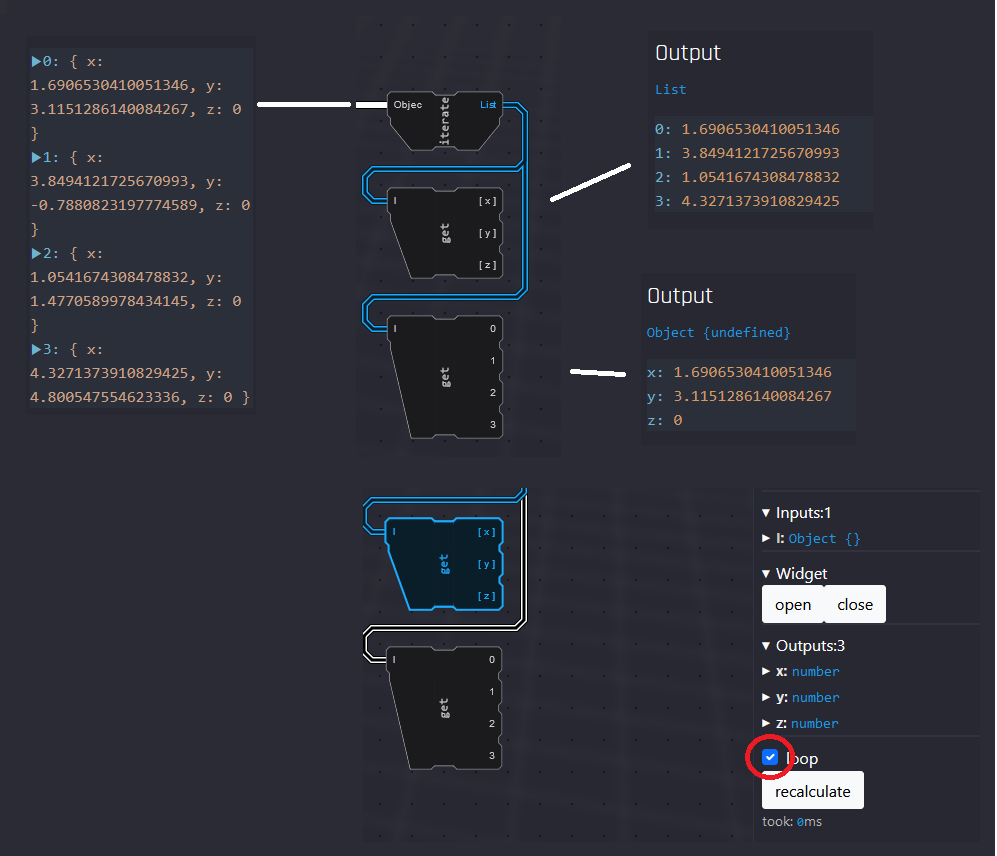
\includegraphics[width=\linewidth]{programming-game.PNG}
  \caption[]{An example of a 'programming game' within Geofront. The 'loop' toggle  indicates if an component should operate on a full list, or operate on all individual items within the list. 
  This can be used to iterate over a 'list of objects' column-wise, or row-wise. This is considered a 'game', since this is not an obvious interaction, and must be learned before properly using Geofront. }
  \label{fig:programming-game}
\end{figure}
 

\subsubsection*{Consistency: When some of the language has been learnt, how much of the rest can be inferred?}

\cite[]{green_usability_1996} notes on the difficulty of defining 'consistency' in language design, and chose to define it as a form of 'predictability'.
Geofront has introduced symbolic distinctions between graphical entities to aid this predictability. 
The biggest is the distinction between \m{operation} and \m{widget} components: 
operations are pure functions with inputs and outputs. 
widgets represent some IO interaction, like an input value, a file, or a web service. 
This way, 'special behavior' is isolated to widgets, making the rest of the script act more predictable. 

In practice, certain inconsistencies within Geofront arise due to the open nature of the plugin system. 
the consistency of geofront is mitigated by a library with a very different notion of naming, or if the library chooses unusual input or output patterns. 
For example, a euclidean, 3D coordinate can be specified as a \m{Vector3} object, a structure, an array of three numbers, or three different x, y, z input parameters.
Then again, it is unclear if inconsistencies between the API's of a language's libraries are to be contributed to the inconsistency of the language as a whole. 

% \textbf{Suggestion for improvement:} Stabilize the api of the Geofront Standard Library.

\subsubsection*{Diffuseness: How many symbols or graphic entities are required to express a meaning?}

Geofront periodically suffers from the same 'Diffuseness' problems \cite{green_usability_1996} adheres to VPLs general. 
That is, sometimes a surprising number of 'graphical entities' / nodes are required to represent a simple statement.  
This is apparent when representing simple mathematical calculations. 

Additionally, the flowchart can only represent linear processes. Many geoprocessing algorithms are iterative and make use of conditionals. These cannot easily be expressed in a Dataflow VPL. As such, these processes must happen within the context of a function, within a 'node'.

A widget evaluating a line of javascript could help improve diffuseness. For now, if a user desires to use dense mathematical statements, or functions with many conditionals and complex iteration, a Geofront Plugin should be created.

% (image of complex / simple mathematical calcluation in javascript and in geofront)

% \textbf{Suggestion for improvement:} These situations could be prevented by allowing scriptable components. 

\subsubsection*{Error- proneness: Does the design of the notation induce 'careless mistakes'?}

There are some errors the user can make  in Geofront that will not be immediately obvious. 
The biggest one is that there are no systems in place preventing large calculations. 
These might freeze up the application. 

To prevent this, the geofront interpreter should have been implemented to run on a separate thread, using a web worker. 
Besides this, in general, many systems are in place preventing errors, such as the type-safety used throughout geofront.
Also, by disallowing cyclical graphs, users cannot create infinite loops accidentally.

\subsubsection*{Hard mental operations: Are there places where the user needs to resort to fingers or pencilled annotation to keep track of what's happening?}

Geofront is developed specifically to prevent "Hard mental operations".
Following the dataflow paradigm explained in \refsec{sec:background:dataflow}, geofront chose to disallows cyclical patterns. 
This greatly reduces the complexity of possible graph configurations, and also causes all in-between results to be immutable or 'final'.
By then allowing these results to be inspected, and allowing the graph to be easily reconfigured, Geofront allows a workflow rooted in experimentation and 'play'.
Users do not need to 'keep track' or 'guess' how things work.
Instead, they can simply experience the behavior, and adjust the behavior until satisfied. 



\subsubsection*{Hidden dependencies: Is every dependency overtly indicated in both directions? Is the indication perceptual or only symbolic?}

The dimension of 'hidden dependencies' is another way the dataflow-paradigm is advantageous. 
The pure functions of a diagram-based VPL like Geofront make the language in general consistent and predictable.
However, there are two exceptions to this rule:
First, the \m{widget} nodes are allowed to produce side-effects, such as opening a window, asking for an input, making a web request, etc. 
These are required to provide geofront with interactive inputs and outputs.
The distinction between \m{widgets} and \m{}

And second, the pureness of functions can only be maintained if all Geofront libraries also exclusively use pure functions. 
There is no fail-safe in place to prevent the usage of a library containing functions with many side-effects. 

\subsubsection*{Premature commitment: Do programmers have to make decisions before they have the information they need?}

In general, Geofront requires almost no premature commitment. 
Or, rather, the level of premature commitment is in line with textual programming languages, in the sense that a user is always somewhat committed to the structure they themselves build. 

One practical way in which Geofront exceeds in this dimension of premature commitment, is that the application does not require a restart upon loading a new library. 
Users can add or remove libraries "on the fly". 
This is unlike any VPL studied at \refsec{sec:related-geovpl} or \refsec{sec:related-webvpl}.

One particular type of commitment users must be aware off, however, is the commitment to using a \ac{VPL} like Geofront in general.
The current version of Geofront does not support compilation to JavaScript yet, which would mitigate this premature commitment. 
% Therefore, 


\subsubsection*{Progressive evaluation: Can a partially-complete program be executed to obtain feedback on 'How am I doing'?}

Yes. 
As explained at the answer for the dimension of 'Hard mental operations', this aspect, together with the ability to inspect parameters, allows a user to 'debug while they write the program'.

\subsubsection*{Role- expressiveness: Can the reader see how each component of a program relates to the whole?}

as the authors of \citet{green_usability_1996} write: "The dimension of role-expressiveness is intended  \\ to describe how easy it is to answer the question 'what is this bit for?'"

One of the ways Geofront addressed this is by making a distinction between nodes possessing pure operations, and nodes producing side effects, like widgets. 

\subsubsection*{Secondary notation: Can programmers use layout, color, other cues to convey extra meaning, above and beyond the 'official' semantics of the language?}

No, Geofront does not offer annotations in its current state, besides the way the nodes are configured on the canvas.  
Geofront does provide visual indicators for types, and for if a cable / variable represents a single item, or a list of items.

This could be improved by providing a way to annotate: to create groups, to write comments, etc. 
Type colors, or some other way to distinguish data based on iconography, would also improve the secondary notation principle.
% \textbf{Suggestion for improvement:} 
% \textbf{Suggestion for improvement:} Type colors would also be nice.

\subsubsection*{Viscosity: How much effort is required to perform a single change?}

Despite these efforts, the 'mouse intensive' interface of vpls like Geofront continues to be a hinder for viscosity.
Certain situations require excessive mouse interaction, like substituting a function with another function, but keeping all inputs the same.
In text, this would be as simple as a non-symbolic renaming of the called function.
In geofront, this requires a lot of reconfiguration of cables. 

Viscosity could be improved by creating special actions in the editor to perform these types of manipulations.  
%  - select multiple inputs, select multiple outputs: connect by height.
% rename node

\subsubsection*{Visibility: Is every part of the code simultaneously visible (assuming a large enough display), or it it at least possible to juxtapose any two parts side-by-side at will? If the code is dispersed, is it at least possible to know in what order to read it?}

All parts of the code are simultaneously visible, and geofront does not offer any way of creating new popups or screens.

% ## Case Studies

% ### Vector
% _Vector data retrieval, transformation, visualization_

% ### Raster 
% _Raster data retrieval, transformation, visualization_

% ### 6. Experiments 
% _Performance benchmark between rust-wasm / cpp-wasm / cgal-cpp-wasm / js / cli usage_

% ## Final 
% _Answer research questions ????_


%%%%%%%%%%%%%%%%%%%%%%%%%%%%%%%%%%%%%%%%%%%%%%%%%%%%%%%%%%%%%%%
%%%%%%%%%%%%%%%%%%%%%%%%%%%%%%%%%%%%%%%%%%%%%%%%%%%%%%%%%%%%%%%
%%%%%%%%%%%%%%%%%%%%%%%%%%%%%%%%%%%%%%%%%%%%%%%%%%%%%%%%%%%%%%%
%%%%%%%%%%%%%%%%%%%%%%%%%%%%%%%%%%%%%%%%%%%%%%%%%%%%%%%%%%%%%%%

% OLD OLD OLD OLD OLD OLD OLD OLD OLD OLD OLD OLD OLD OLD OLD


% We group the requirements listed at \refsec{sec:method-one} in a group of base features,
% a group of dataflow features, and a group of geometry features.


% \section{Experiments}

% \subsection{ Web Mapping Service }
% -> could work, must be captured in component
% -> streaming question

% \subsection{ Open Street Map }
% -> could be hooked up to the geojson viewer



% \section{ Performance }
% \subsection{Vector 3D}

% ....

% \subsection{Raster}

% ....

% \subsection{Geo features}

% ....


%%%%%%%%%%%%%%%%%%%%%%%%%%%%%%%%%%%%%%%%%%%%%%%%%%%%%%%%%%%%%%%%%%%%%%%%%
% \section{Use Case: Educational Sandbox}
% \begin{lstlisting}
% WHAT: 
%  - show the behaviour of a simple ransac algorithm, fitting a plane through 
%    a point cloud
%  - show it beharivourly: show in-between steps
%  - make parameters ajustable (number of high scores, minimum high score, 
%    number of tries, etc.)
%  - add least squares adjustment, and compare.

% SIMILAR EXAMPLES: 
%  - the geometric predicates explanation 
%  (https://observablehq.com/@mourner/non-robust-arithmetic-as-art)
%  - 

% ASSESS ON: 
%  - educational value
%  - ease of usage (the promise of **Criterium A**)
 
% ASSESSMENT (hypothesis): 
%  + indeed very insightful for analying the behaviour 
%    and operation of certain 
%    algorithms & parameters. Not many applications can show 
%    this level of insight. 
%  + feature B can be used to strip the tool down 
%    to the bare minimum,   helping 
%    with not overwhelming the user with features

%  - This VPL is not easy to operate. 
%    It remains difficult to communicate what needs to 
%    be done, how things work. This is not an expert tool, 
%    but also not a beginners' tool.
%  - No built-in tutorialization
%  - hard to discover the code underneath, 
%    obfuscating the link between process and code.

% \end{lstlisting}

% %%%%%%%%%%%%%%%%%%%%%%%%%%%%%%%%%%%%%%%%%%%%%%%%%%%%%%%%%%%%%%%%%%%%%%%%%
% \section{Use Case: Web Demo Environment}
% \begin{lstlisting}
%     WHAT:
%      - Show the startin delaunay triangulator
%      - Accept user-submitted Laz files as input
%        - filter the ground
%      - Accept a randomly generated point cloud based on perlin noise.
%      - Visualize the generated mesh, and make it available for download

%     EXAMPLES: 
%      - hugo's demo
    
%      ASSESS ON:
%      - **Criterium B**: extendability: 
%        - how does foreign and native codebases interact? 
%      - clarity
%      - reproducibility
%      - performance
%      - scope (raster / vector / 2D / 3D)

%     JUDGEMENTS (hypothesis): 
%      + Clarity is fine
%      + Reproducability is 
%      + Performance is decent

%      ~ clarity is fine, vpl allows users to 'play around' and try
%        different configurations, even run their own data through the
%        demonstrated functions

%      - Application is less suited for 2D 
    
% \end{lstlisting}


% \section{Use Case: Geoprocessing Environment}%%%%%%%%%%% SECTION
% \begin{lstlisting}

%     WHAT:
%       - Query an area of a point cloud with a polygon
%       - turn that area of points into a triangulation
%       - turn triangulation into isocurves
%       - save this as a geojson
%       - turn this whole thing into a function, which takes a PC, 
%         polygon and isocurve range, and spits out the geojson
%       - share this using a link
%       - turn this into an app?
%       - turn this into a script?

%     EXAMPLES: 
%      - 

%      ASSESS ON:
%      - **Criterium C**: Publicability:
%        - the ability to operationalize the application 
%        - can it be used by end-users? clarity? too much clutter

%     JUDGEMENTS (hypothesis): 
%       ~ sharing by link is possible, but for end-user usage, 
%         its very cluttered 
%       ~ compiling to js only partially works
%       ~ compiling into an app is not possible, but 
%         since everything runs client-side, it could be implemented. 

% \end{lstlisting}
